%pdflatex --shell-escape scap_benchmark_dl_training_results
%biber scap_benchmark_dl_training_results

\PassOptionsToPackage{hyphens}{url}
\documentclass[compress,aspectratio=169]{beamer}

\usepackage[official]{eurosym}
\usepackage{multirow}
\setlength{\marginparwidth}{2cm}
\usepackage{todonotes}
\presetkeys{todonotes}{inline}{}
\usepackage[style=verbose,backend=biber,style=authoryear, citestyle=authoryear ]{biblatex}
\setbeamertemplate{bibliography item}{\insertbiblabel} % Ensure that cite labels appear in references section
\addbibresource{ref.bib}
\usepackage{../assets/beamerthemeGoettingen} % make sure the theme file is on this path
\graphicspath{{../}{../assets/}}
\usepackage{caption}
\usepackage{booktabs}

\usepackage{listings}

\hypersetup{
    colorlinks,
    citecolor=black,
}

\newcommand{\source}[1]{\par\begin{textblock*}{6cm}(1cm,8cm)
    \begin{beamercolorbox}[wd=\paperwidth,ht=0.5cm,right]{framesource}
        \usebeamerfont{framesource}\usebeamercolor[fg]{framesource} \centering\tiny {#1}
    \end{beamercolorbox}
\end{textblock*}}


% listing / code
\usepackage{minted}
\usemintedstyle{tango}
% Box listing / code
\usepackage{tcolorbox}

% Box listing / code style 
% These options will be applied to all `tcolorboxes`
\tcbset{%
    noparskip,
    colback=gray!5, %background color of the box
    colframe=gray!20, %color of frame and title background
    coltext=black, %color of body text
    coltitle=black, %color of title text 
    fonttitle=\tiny,
    alerted/.style={coltitle=red, 
                     colframe=gray!40},
    example/.style={coltitle=black, 
                     colframe=green!20,             
                     colback=green!5},
    }

\lstset{literate=%
    {Ö}{{\"O}}1
    {Ä}{{\"A}}1
    {Ü}{{\"U}}1
    {ß}{{\ss}}1
    {ü}{{\"u}}1
    {ä}{{\"a}}1
    {ö}{{\"o}}1
    {~}{{\textasciitilde}}1
}

\usepackage{csquotes} % For \enqoute{}
\usepackage{hyperref}

% --- document configuration ---
\newcommand{\mytitle}{Benchmarking tree species classification\\with synthetic data and deep learning}     
% Leave empty for no subtitle
\newcommand{\mysubtitle}{State of the art and plan for Scalable Computing Systems and Applications in AI, Big Data and HPC}   
\newcommand{\myauthor}{Hauke Kirchner}
\newcommand{\myauthorurl}{\href{http://www.overleaf.com}{Something 
Linky}}
\newcommand{\myvenue}{Göttingen}
% For example, use \today
\newcommand{\mydate}{24.11.2022}
% For example, Institute for Computer Science / GWDG
\newcommand{\myinstitute}{GWDG - AG Computing}
% Leave empty for no footer image
\newcommand{\myfooterimage}{}           
\newcommand{\mygrouplogo}{}
% Images must be enabled manually under title page \titleLogo
% Adjust position and width manually for fewer images
\newcommand{\mytitleimageone}{}         
\newcommand{\mytitleimagetwo}{}        
\newcommand{\mytitleimagethree}{}

% --- title page ---
\title{\Large \mytitle}
\venue{\myvenue}
\date{\mydate}
\subtitle{\mysubtitle}
%\authorURL{\myauthorurl}
\author{{\myauthor}}
\authorFooter{\myauthor \hspace{0.3cm} \includegraphics[height=1em]{\myfooterimage}}
\institute{\myinstitute}
\groupLogo{\includegraphics[width=2cm]{\mygrouplogo}}
\titleLogo{
%\includegraphics[height=2.7cm]{\mytitleimageone}
%\includegraphics[height=2.7cm]{\mytitleimagetwo}
%\includegraphics[height=2.7cm]{\mytitleimagethree}
}

\setbeamertemplate{footline}[text line]{
\begin{beamercolorbox}[sep=0.5em,wd=\paperwidth,leftskip=0.2cm,rightskip=0.1cm]{footlinecolor}
\myauthor \hfill \insertVenue \hfill \insertframenumber\,/\,\ref{pg:lastpage}
\end{beamercolorbox}
}

\begin{document}

\begin{frame}[plain]
	\titlepage
\end{frame}

\begin{frame}[t]{Table of contents}
  \tableofcontents[subsectionstyle=hide/hide]
\end{frame}

% --- slides begin ---

\section{Motivation}

\begin{frame}{Why is it important to benchmark the training process of neural networks?}

    \begin{columns}
        \begin{column}{0.5\textwidth}
            \begin{block}{\centering Training speed}
                \centering
                \vspace{3em}
                
\includegraphics[width=0.3\textwidth]{assets/speed_FILL0_wght400_GRAD0_opsz48.png}
            \end{block}
        \end{column}
        \begin{column}{0.5\textwidth}
            \begin{block}{\centering Energy efficiency}
                \centering
                \vspace{3em}
                
\includegraphics[width=0.3\textwidth]{assets/electric_bolt_FILL0_wght400_GRAD0_opsz48}
            \end{block}
        \end{column}
    \end{columns}

\end{frame}

\begin{frame}{Training speed 
              \begin{tabular}{@{}c@{}}
                  
\includegraphics[width=0.05\textwidth]{assets/speed_FILL0_wght400_GRAD0_opsz48.png}
              \end{tabular}
              }

    \vspace{-3em}

    \begin{columns}
        \begin{column}{0.6\textwidth}
            \begin{itemize}
                \item training of neural networks is computationally intensive
                \item[$\hookrightarrow$] workflow needs to be optimized for available hardware
                    \begin{itemize}
                        \item How to make good use of clusters with heterogenous hardware?
                        \item How many GPUs are worth requesting?
                    \end{itemize}
                    \vspace{2em}
                \item[$\Rightarrow$] optimization for available accelerators is critical in ML/DL
            \end{itemize}
        \end{column}
        \begin{column}{0.4\textwidth}
            \vspace{-1em}
            \begin{figure}
                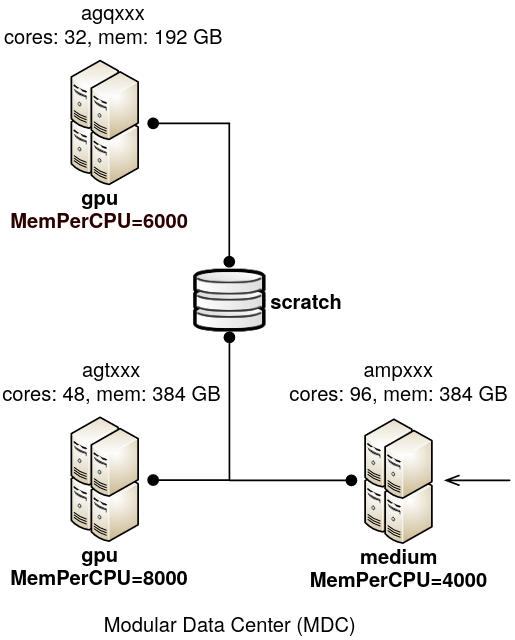
\includegraphics[width=0.9\textwidth]{assets/gwdg_scc.png}
                \caption*{Structure and resources of a part of the Scientific Compute Cluster.}
            \end{figure}
        \end{column}
    \end{columns}

    \source{Image source: Adapted from \url{https://www.gwdg.de/web/guest/hpc-on-campus/scc}, accessed on: 09.11.2022}
\end{frame}

\begin{frame}{Energy efficiency 
              \begin{tabular}{@{}c@{}}
                  
\includegraphics[width=0.05\textwidth]{assets/electric_bolt_FILL0_wght400_GRAD0_opsz48}
              \end{tabular}
              }



    \begin{columns}
        
        \begin{column}{0.6\textwidth}
            \begin{itemize}
                \item for different neural networks, the required energy ranges from relatively low demands (finetuning) to very high demands (training of a complex network)
                \item depends on used hardware and energy source
                \item[$\Rightarrow$] As deep learning is emerging in several fields, the impact on energy consumption and consequently, our climate is growing
            \end{itemize}
        \end{column}

        \begin{column}{0.4\textwidth}
            \vspace{-3.5em}
            \centering
            \begin{figure}
            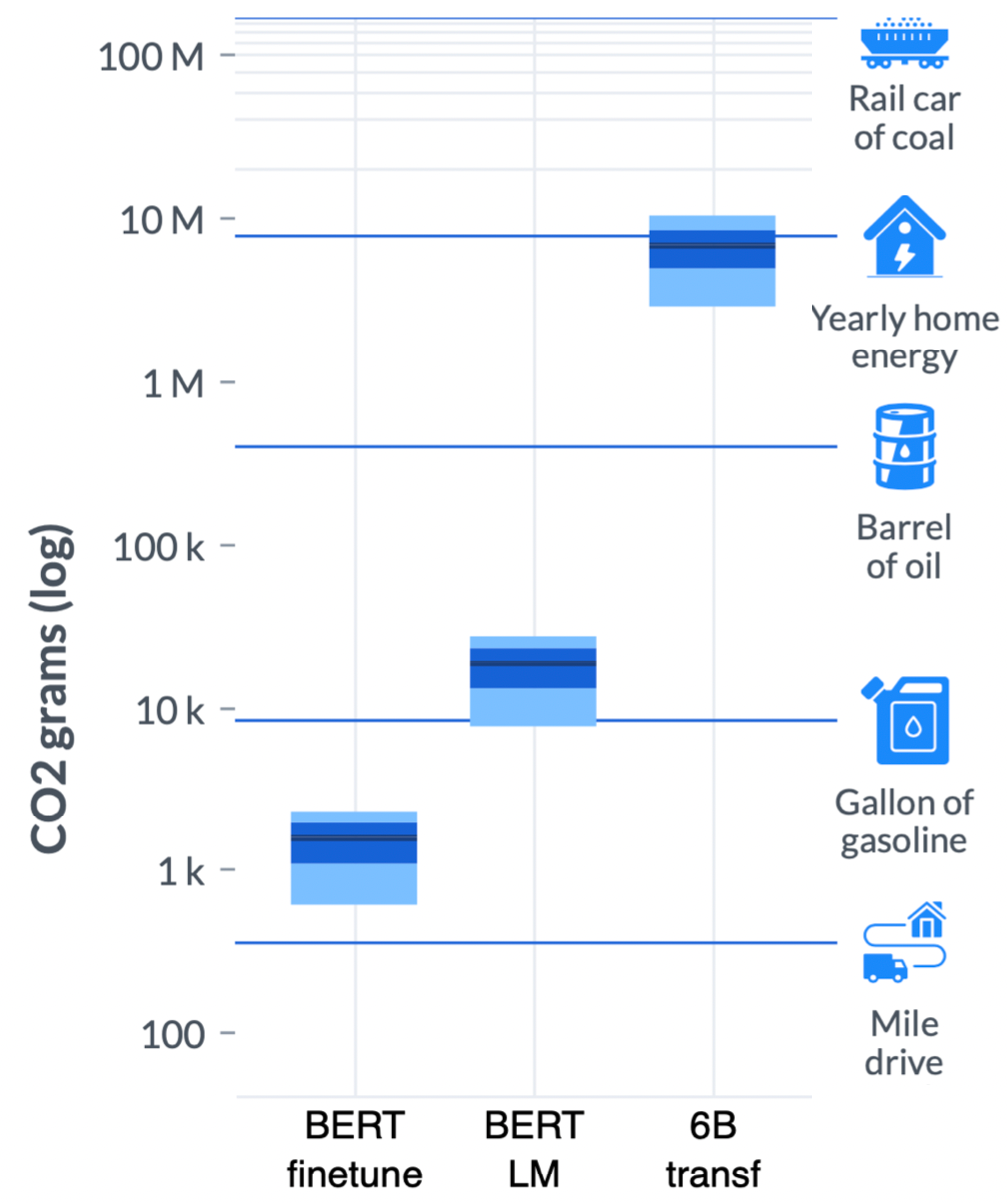
\includegraphics[width=\textwidth]{assets/20220610_dodge_measuring-the-carbon-intensity-of-ai-in-cloud-instances-fig2-bert.png}
            \caption*{$CO_2$ Relative Size Comparison}
            \end{figure}
            \source{Image source: Adapted from \cite{20220610_dodge_measuring-the-carbon-intensity-of-ai-in-cloud-instances}}
            
        \end{column}
    \end{columns}



\end{frame}

\begin{frame}{Use case}
    \begin{columns}
        \begin{column}{0.5\textwidth}
            \vspace{-1em}
            \begin{block}{Tree species classification from lidar}
                \begin{itemize}
                    \item monitoring of tree species is essential for forest restructuring towards more resilient forests in changing environments under climate change condition~\footnote{\tiny{\url{https://www.umweltbundesamt.de/angepasster-waldumbau}}}
                    \item lidar is already in use for forest inventories (\cite{white_2016_als-forest-inventory})
                    \item Problem: lack of pre-trained models
                \end{itemize}
            \end{block}

        \end{column}
        \begin{column}{0.5\textwidth}
                \centering
                \vspace{-3em}
                \begin{figure}
                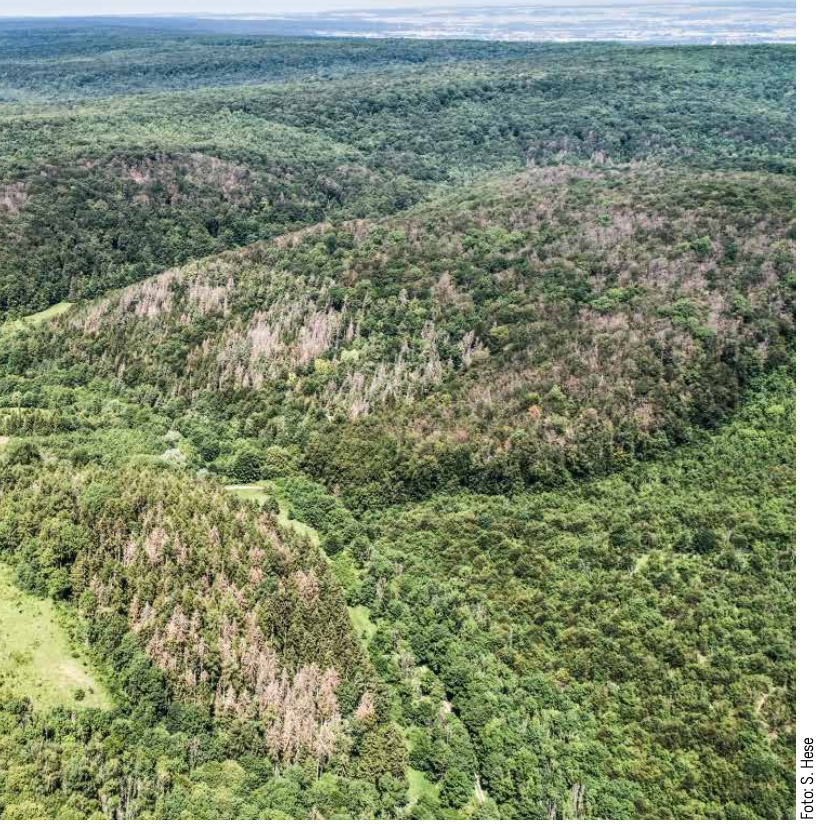
\includegraphics[width=0.9\textwidth]{assets/beech_drought}
                \caption*{Spruce and beech stand close to the national park "Hainich".}
                \end{figure}
                \source{Image source: Adapted from \cite{henkel_2021}}
        \end{column}
    \end{columns}
\end{frame}

\section{Methods}
\sectionIntroHidden % Show an outline of the current section with hidden subsections
%\sectionIntro % Show an outline of the current section with subsections

\begin{frame}{Workflow}
    \begin{columns}
        \begin{column}{0.5\textwidth}

            \begin{block}{Pre-training with synthetic data}
                \begin{enumerate}
                    \item scene generation with Arbaro\footnote{\tiny{\url{https://github.com/wdiestel/arbaro}}}
                    \item synthetic lidar data is generated with the  lidar operations simulator Helios++ (\cite{9906068})
                    \item pre-training of PointNet, which is a very popular architecture for point cloud analysis (\cite{pointnet})
                \end{enumerate}
            \end{block}

        \end{column}
        \begin{column}{0.5\textwidth}
                \centering
                \vspace{-4em}
                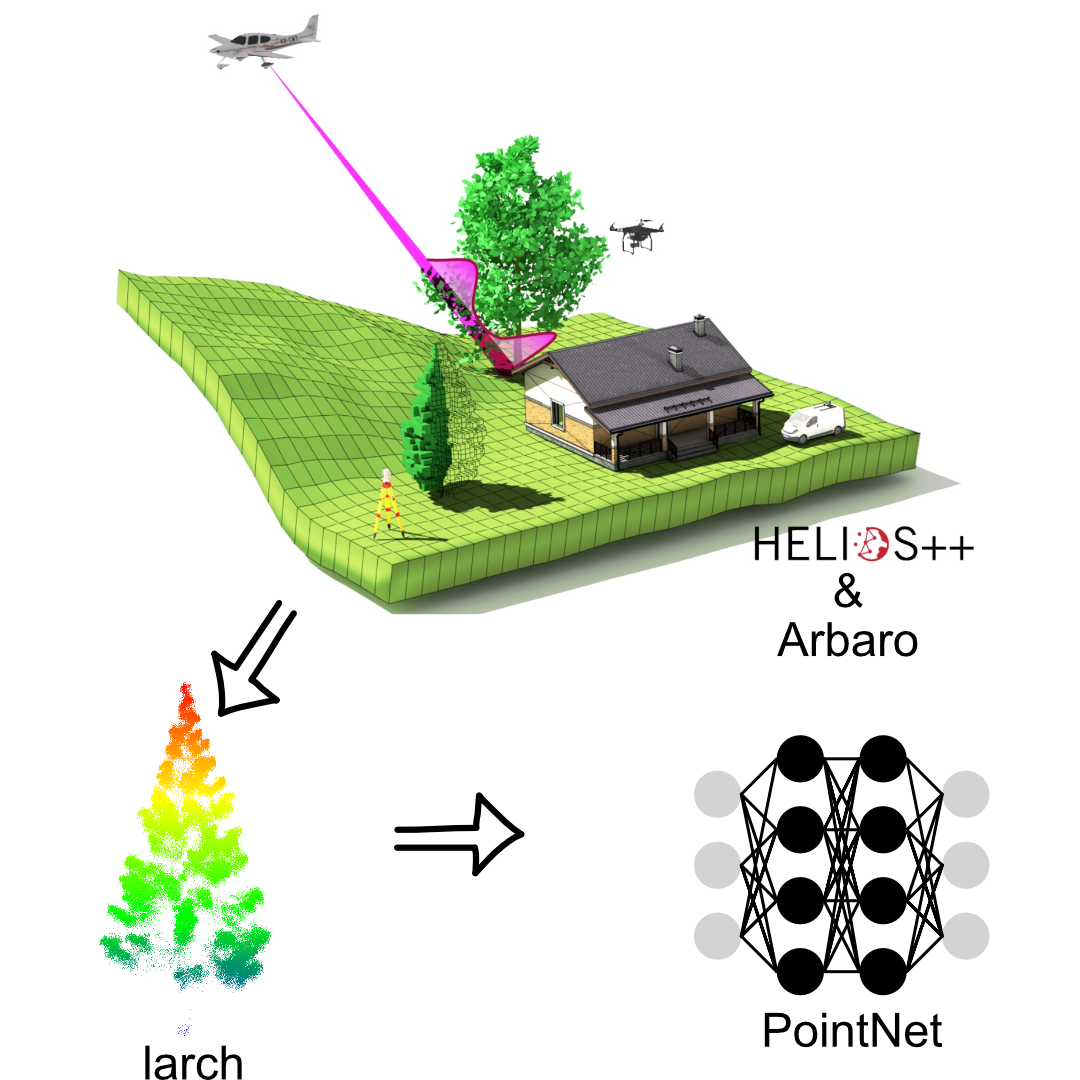
\includegraphics[width=\textwidth]{assets/workflow_synthetic_data}
                \source{Image source: Adapted from \cite{9906068}}
        \end{column}
    \end{columns}
\end{frame}

\begin{frame}{Metrics}

% Please add the following required packages to your document preamble:
% \usepackage{booktabs}
% \usepackage{multirow}
\begin{table}[]
\begin{tabular}{@{}ll@{}}
\toprule
metric                                                                                 & purpose                        \\ \midrule
Execution time                                                                         & \multirow{2}{*}{traditionally} \\
FLOPS                                                                                  &                                \\ \midrule
Throughput: $\frac{images}{sec}$                                                       & with the advent of GPUs        \\ \midrule
Time to Accuracy (TTA)                                                                 & \multirow{2}{*}{deep learning} \\
\begin{tabular}[c]{@{}l@{}}Average Time to \\ Multiple Thresholds (ATTMT)\end{tabular} &                                \\ \bottomrule
\end{tabular}
\end{table}


\source{Image source: Adapted from \url{https://snehilverma41.github.io/Metrics_ML_FastPath19.pdf}}

\end{frame}


\section{Tools}
\sectionIntroHidden

\begin{frame}{Tools - Overview}

% Please add the following required packages to your document preamble:
% \usepackage{booktabs}
% \usepackage{multirow}
\begin{table}[]
\begin{tabular}{@{}lll@{}}
\toprule
tool                              & metrics                                                                                & scope                    \\ \midrule
\href{https://pytorch.org/tutorials/intermediate/tensorboard_profiler_tutorial.html}{PyTorch Profiler With TensorBoard} & \begin{tabular}[c]{@{}l@{}}performance metrics\\ (e.g. time, memory)\end{tabular}      & \multirow{2}{*}{PyTorch} \\
\href{https://github.com/facebookresearch/fvcore}{fvcore}                      & FLOPS                                                                                  &                          \\ \midrule
\href{https://www.intel.com/content/www/us/en/developer/tools/oneapi/vtune-profiler.html}{Vtune}                             & \multirow{2}{*}{\begin{tabular}[c]{@{}l@{}}general\\ performance metrics\end{tabular}} & Intel-only               \\
\href{https://github.com/RRZE-HPC/likwid}{likwid}                            &                                                                                        & general                  \\ \bottomrule
\end{tabular}
\end{table}



\begin{itemize}
    \item[$\Rightarrow$] different tools for different use cases
    \item[$\Rightarrow$] Vtune and likwid can profile all kind of applications
    \item[$\Rightarrow$] here I will focus on profiling tools optimized for PyTorch
\end{itemize}

\end{frame}

\begin{frame}{PyTorch Profiler With TensorBoard}
    \vspace{-1em}
    \begin{center}
    \begin{figure}
        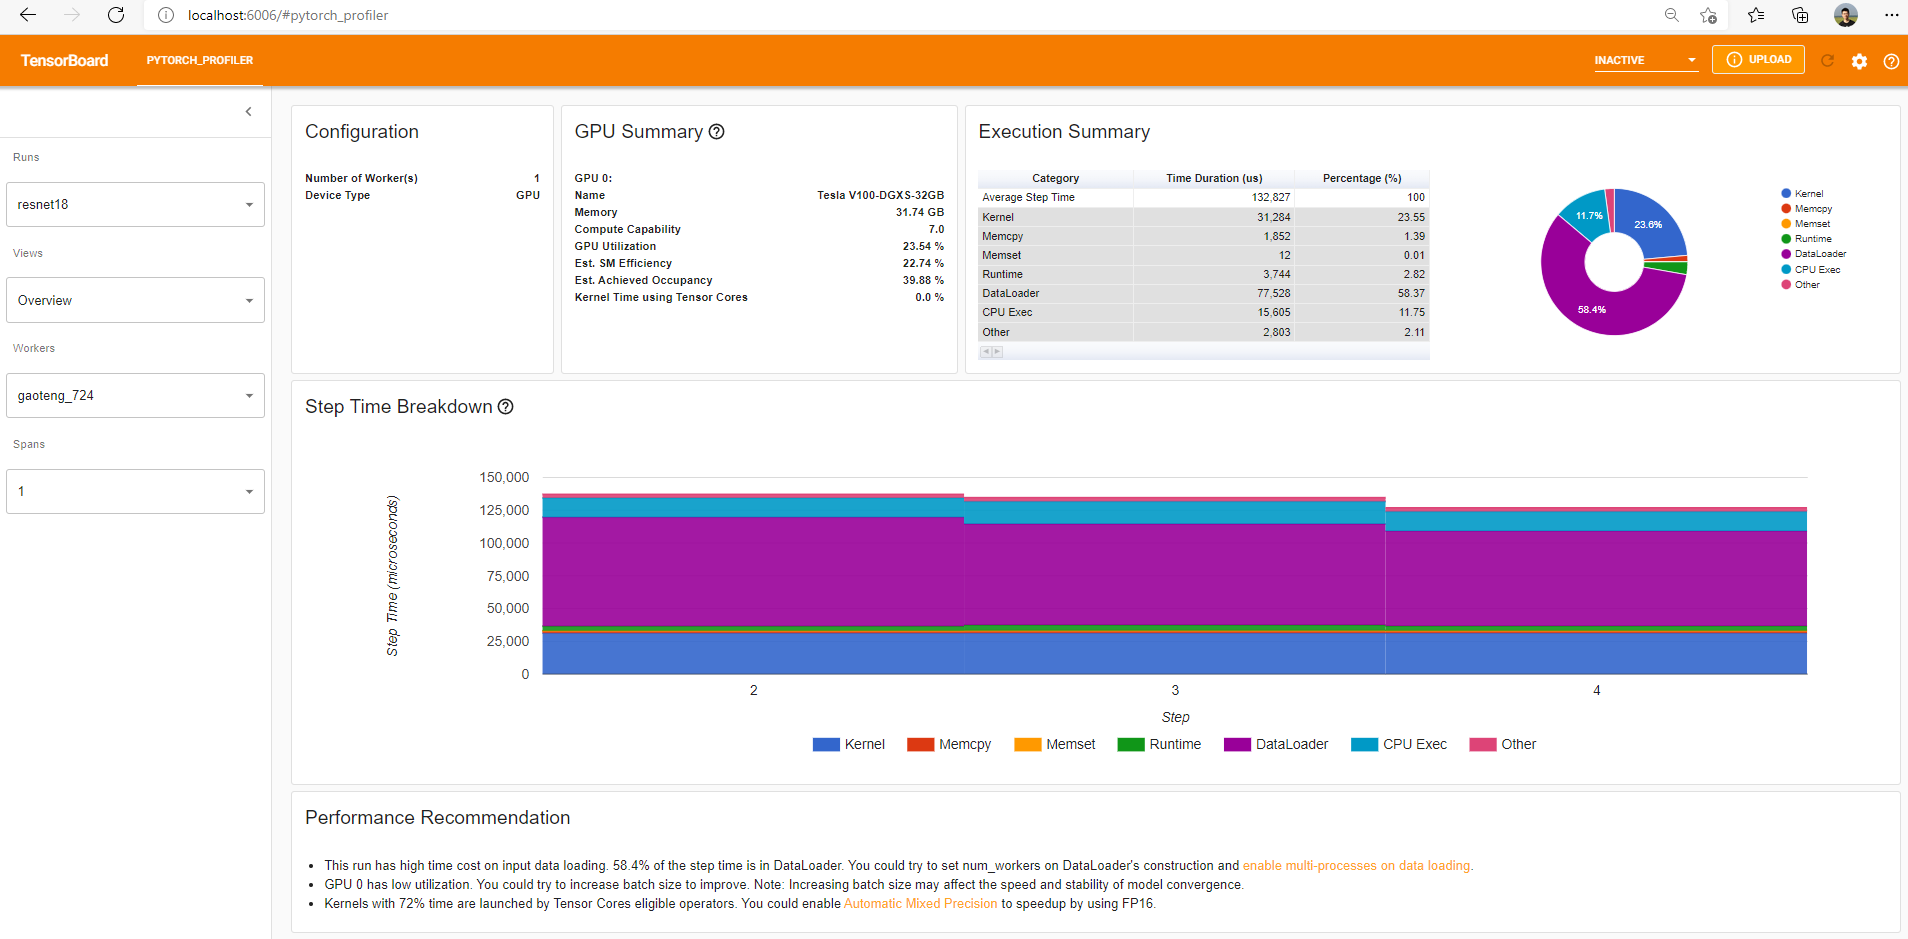
\includegraphics[width=1\textwidth]{assets/profiler_overview1}
    \end{figure}
    \end{center}
\source{Image source: \url{https://pytorch.org/tutorials/intermediate/tensorboard_profiler_tutorial.html}, accessed on: 22.11.2022}

\end{frame}

\begin{frame}{PyTorch Profiler With TensorBoard}
    \vspace{-1em}
    \begin{center}
    \begin{figure}
        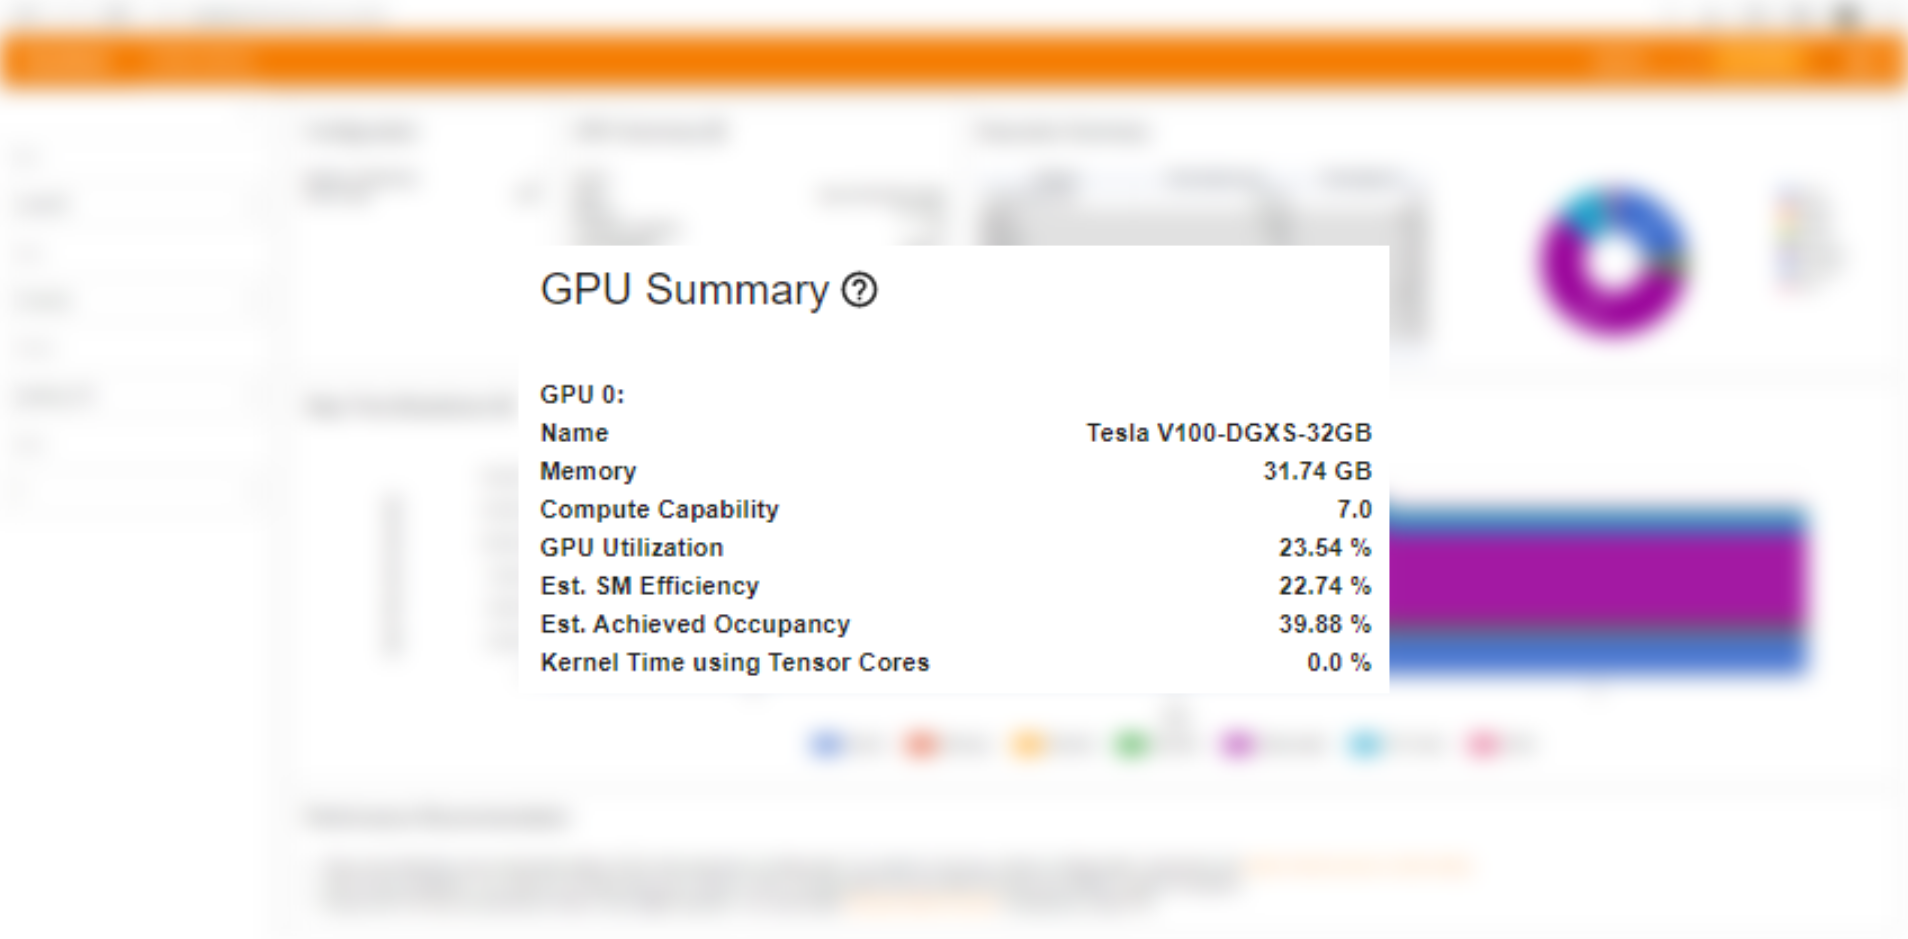
\includegraphics[width=1\textwidth]{assets/profiler_overview_gpu_summary}
    \end{figure}
    \end{center}
\source{Image source: Adapted from \url{https://pytorch.org/tutorials/intermediate/tensorboard_profiler_tutorial.html}, accessed on: 22.11.2022}

\end{frame}

\begin{frame}{PyTorch Profiler With TensorBoard}
    \vspace{-1em}
    \begin{center}
    \begin{figure}
        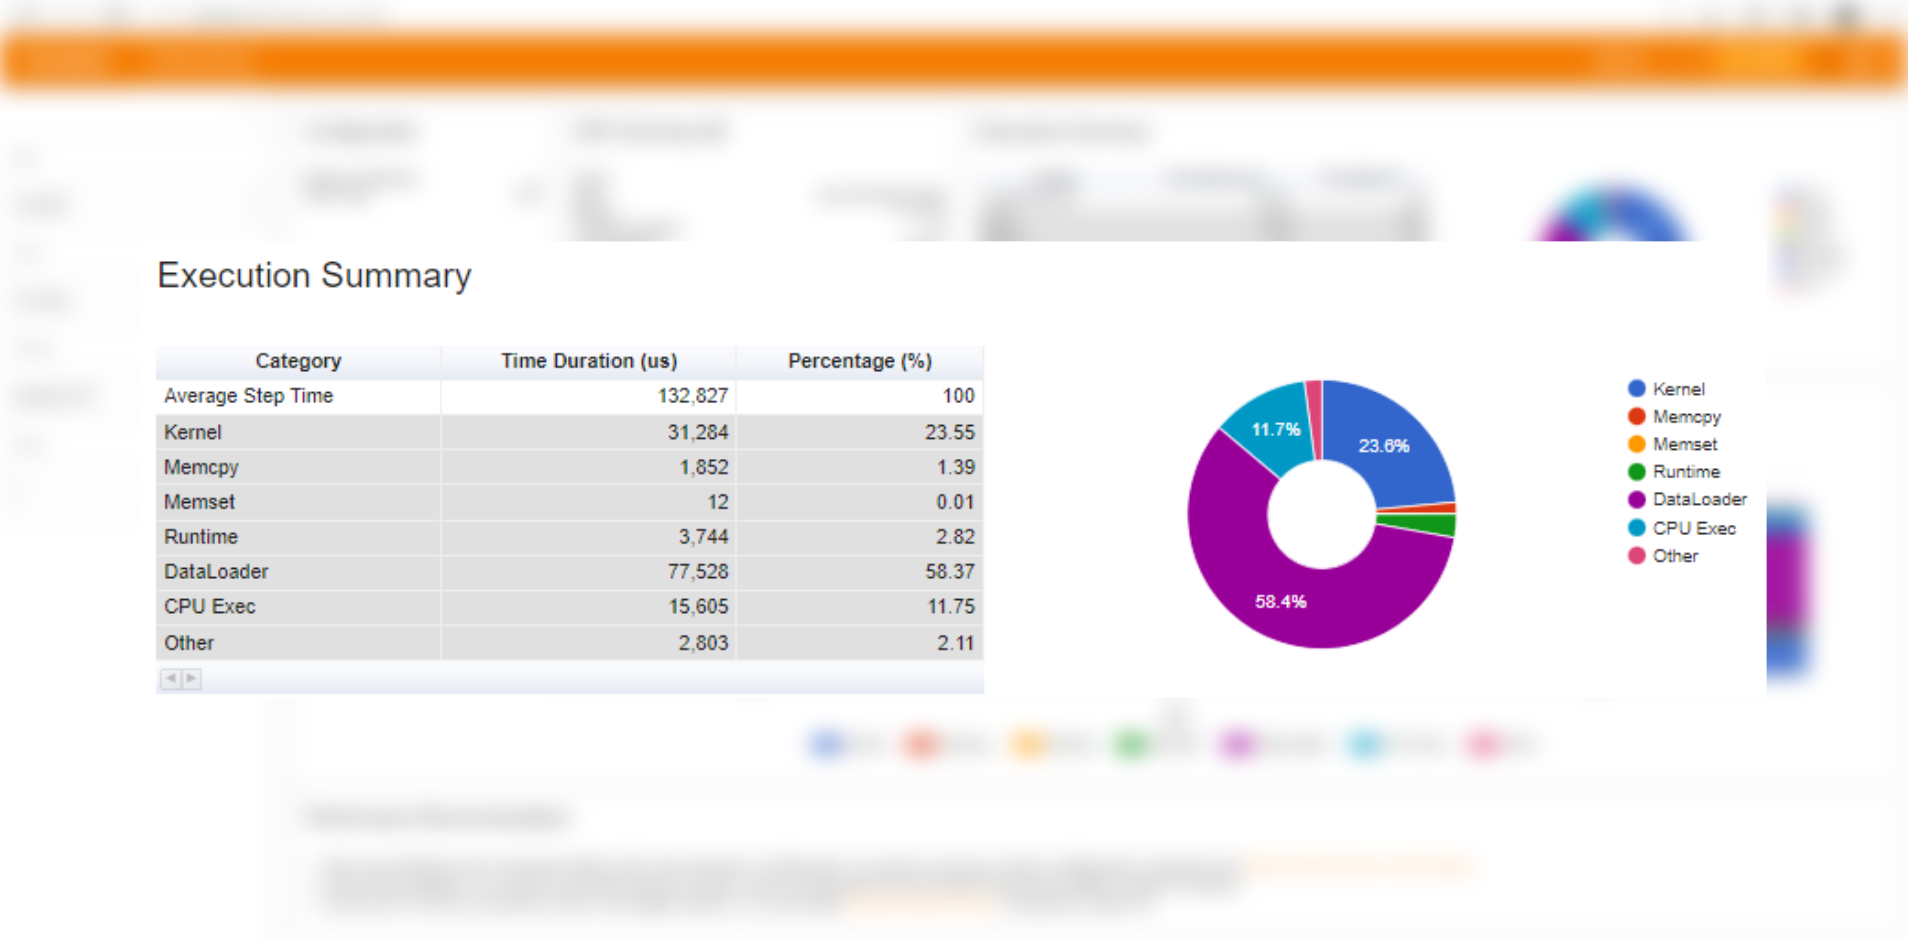
\includegraphics[width=1\textwidth]{assets/profiler_overview_execution_time}
    \end{figure}
    \end{center}
\source{Image source: Adapted from \url{https://pytorch.org/tutorials/intermediate/tensorboard_profiler_tutorial.html}, accessed on: 22.11.2022}

\end{frame}

\begin{frame}{PyTorch Profiler With TensorBoard}
    \vspace{-1em}
    \begin{center}
    \begin{figure}
        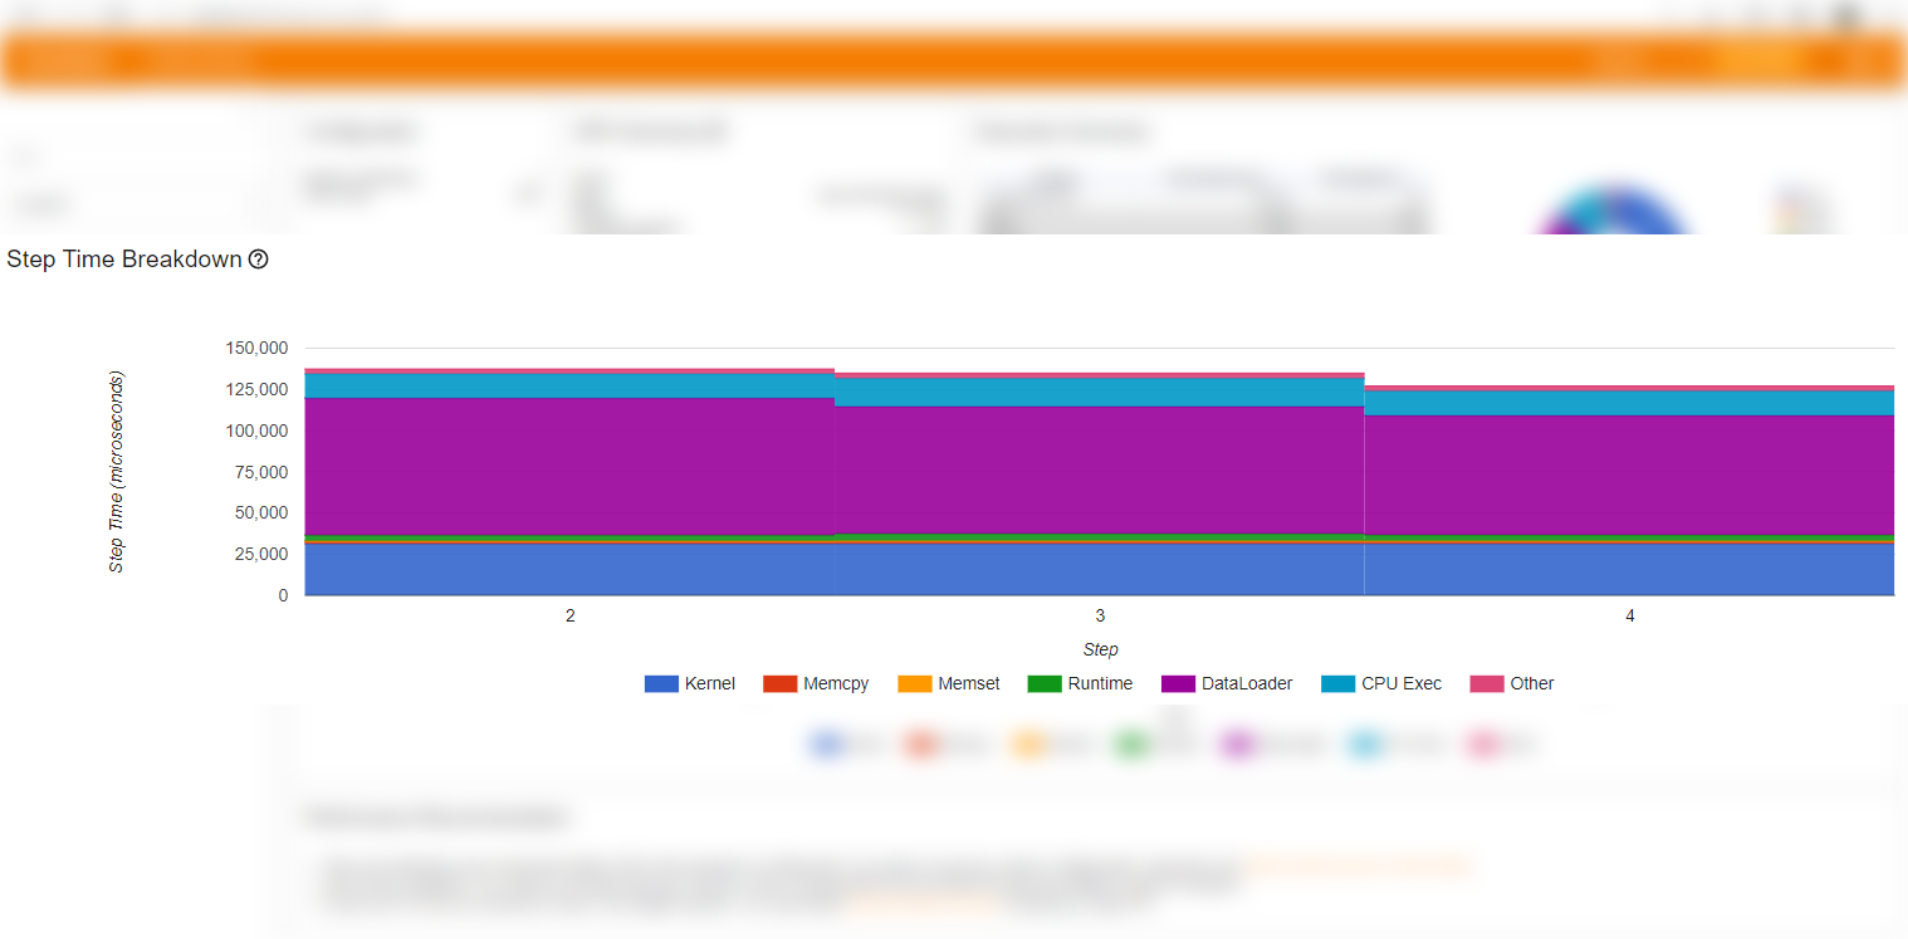
\includegraphics[width=1\textwidth]{assets/profiler_overview_step_time_breakdown}
    \end{figure}
    \end{center}
\source{Image source: Adapted from \url{https://pytorch.org/tutorials/intermediate/tensorboard_profiler_tutorial.html}, accessed on: 22.11.2022}

\end{frame}

\end{frame}

\begin{frame}{PyTorch Profiler With TensorBoard}
    \vspace{-1em}
    \begin{center}
    \begin{figure}
        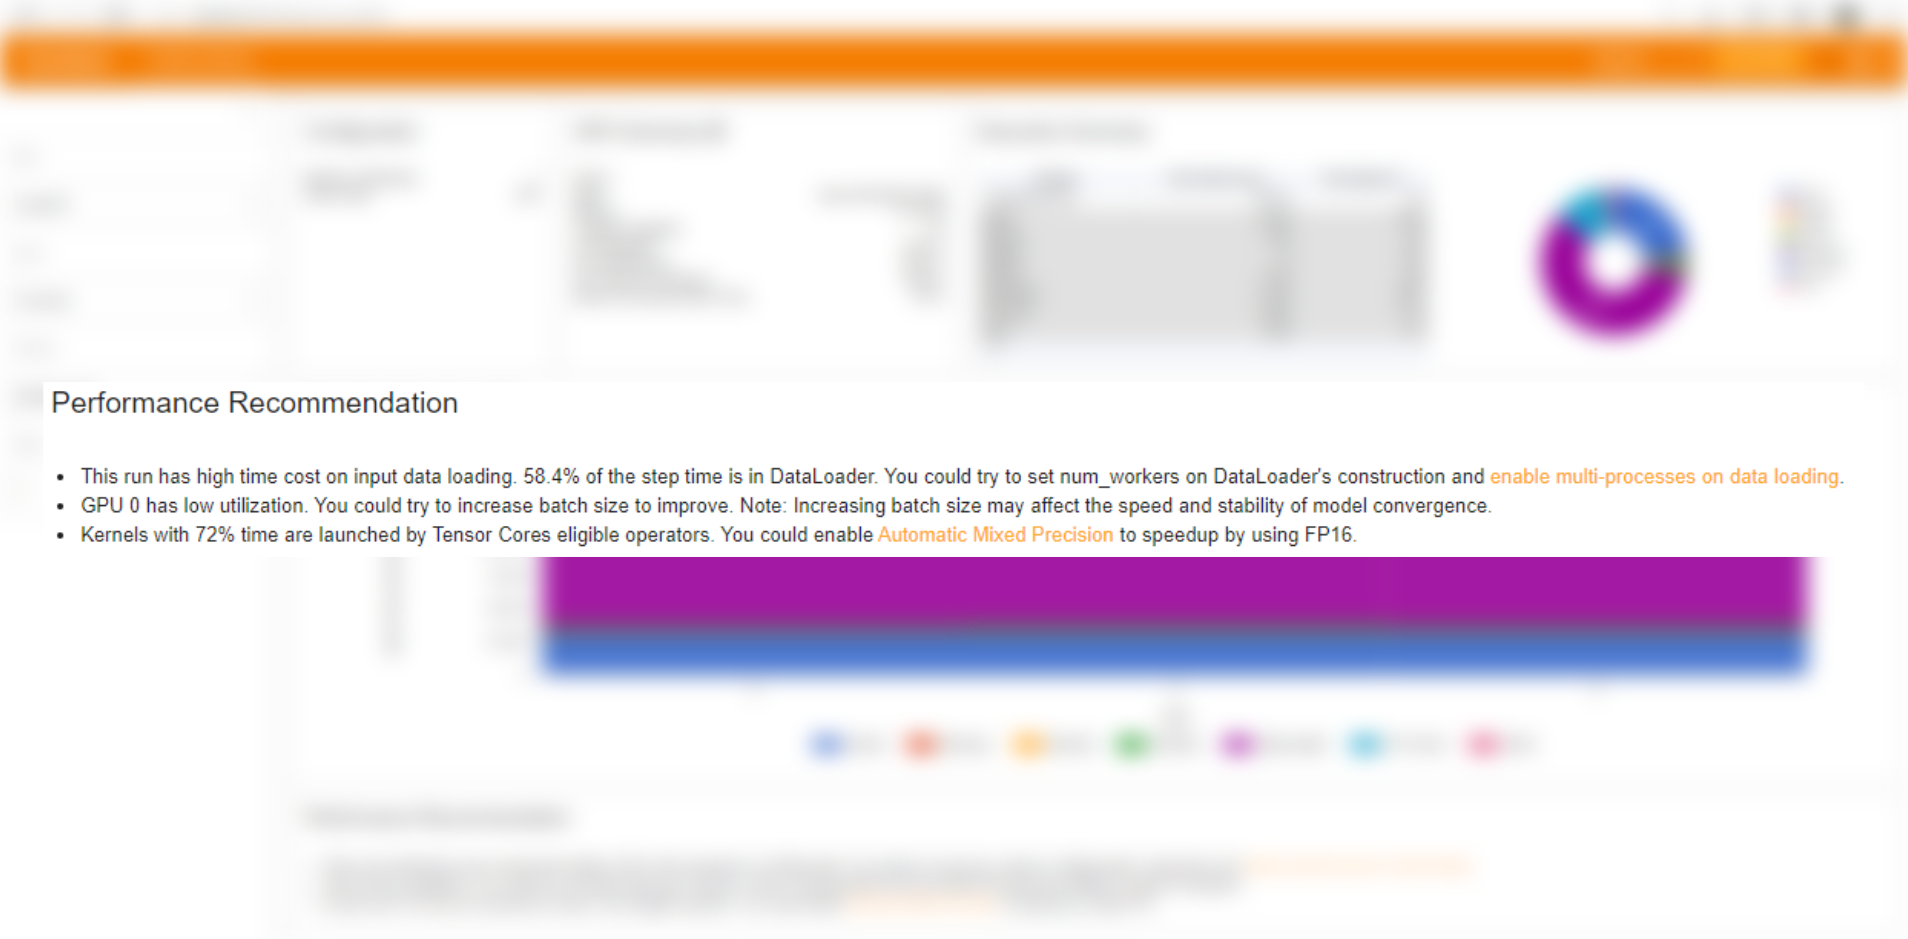
\includegraphics[width=1\textwidth]{assets/profiler_overview_performance_reccomondation}
    \end{figure}
    \end{center}
\source{Image source: Adapted from \url{https://pytorch.org/tutorials/intermediate/tensorboard_profiler_tutorial.html}, accessed on: 22.11.2022}

\end{frame}

\begin{frame}{fvcore - Flop Counter for PyTorch Models}
    \vspace{-1em}
    \begin{center}
    \begin{figure}
        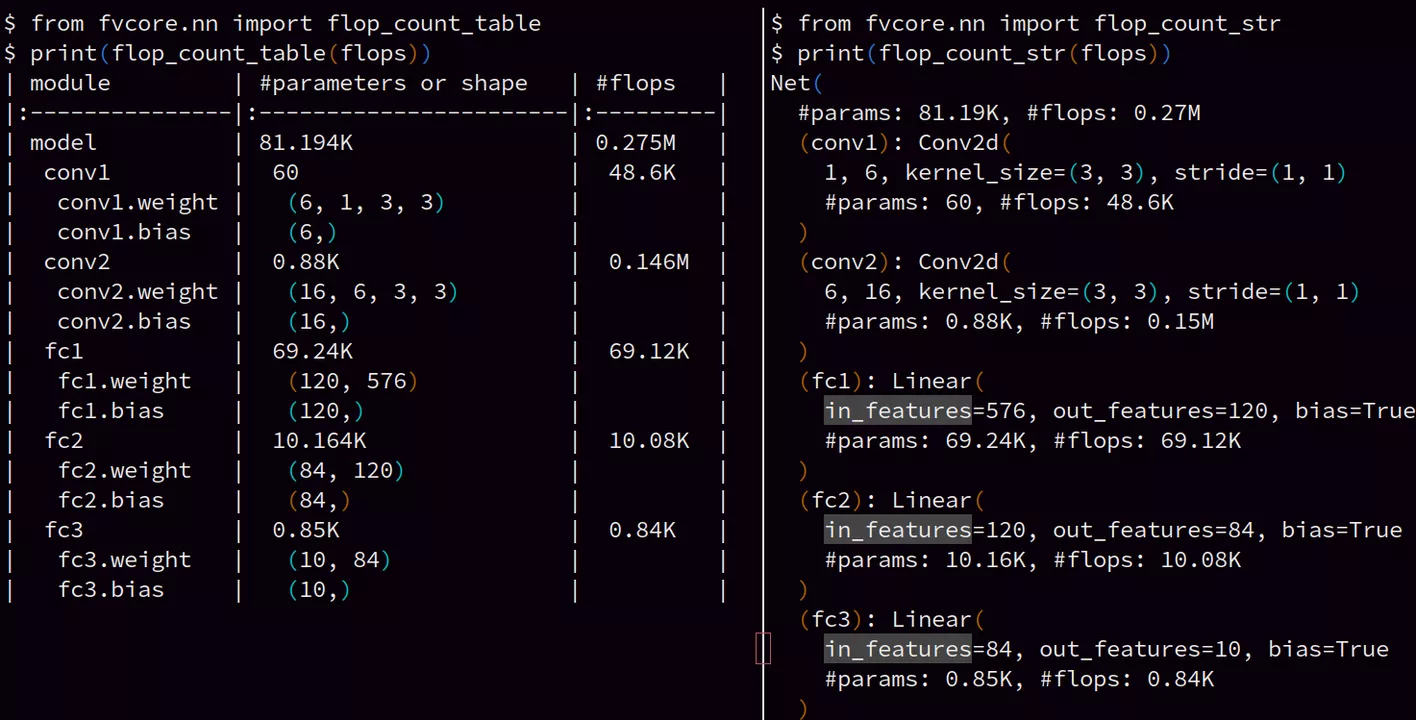
\includegraphics[width=0.9\textwidth]{assets/flop_counter_print}
    \end{figure}
    \end{center}
\source{Image source: \url{https://github.com/facebookresearch/fvcore/blob/main/docs/flop_count.md}, accessed on: 22.11.2022}

\end{frame}

\section{Research Goals}

\begin{frame}{Research Goals}

\begin{itemize}
    \item Identify \textbf{profiling tools} that can help to \textbf{optimize an existing PyTorch workflow}.
    \item As this approach should help scientists, the \textbf{usibility is of high importance}. The simplest tool for doing the job is preferred.
    \item In contrast to training benchmark suites, such as MLPerf, I do not focus on benchmarking hardware but on optimizing an existing PyTorch workflow (viewpoint of a scientist)
\end{itemize}

\end{frame}

\section{Results}

\begin{frame}{First attempt using PyTorch Profiler}
    \begin{center}
    \begin{figure}
        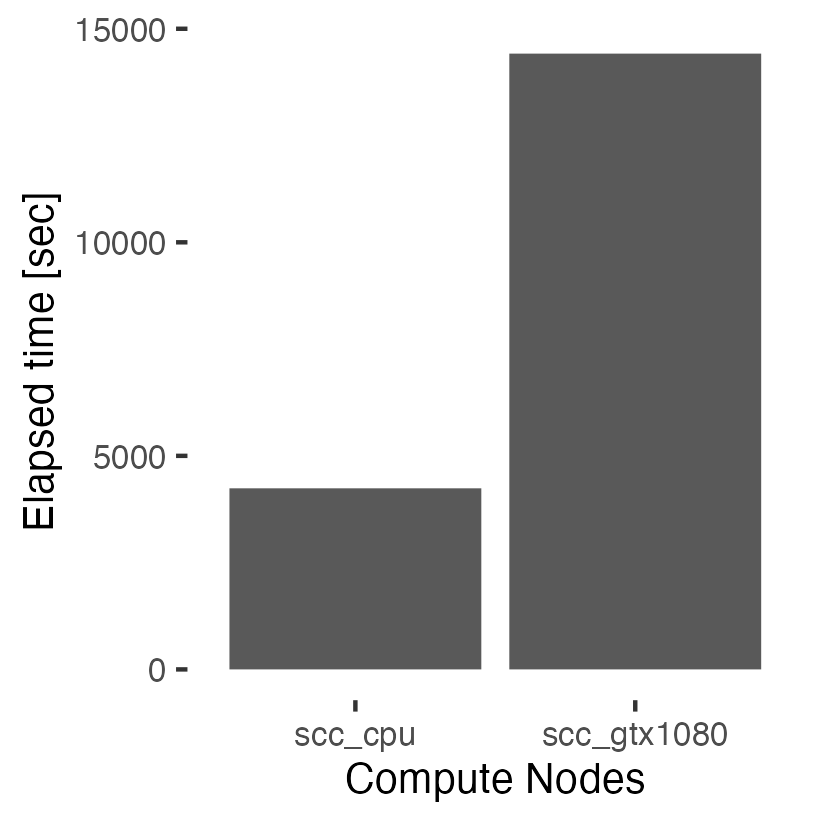
\includegraphics[width=0.5\textwidth]{../../data/sacct_barplot_by_nodes_profiler-torch_sample-points}
    \end{figure}
    \end{center}
\end{frame}

\begin{frame}{Trying to use the PyTorch Profiler to find the reason}
    \begin{center}
    \begin{figure}
        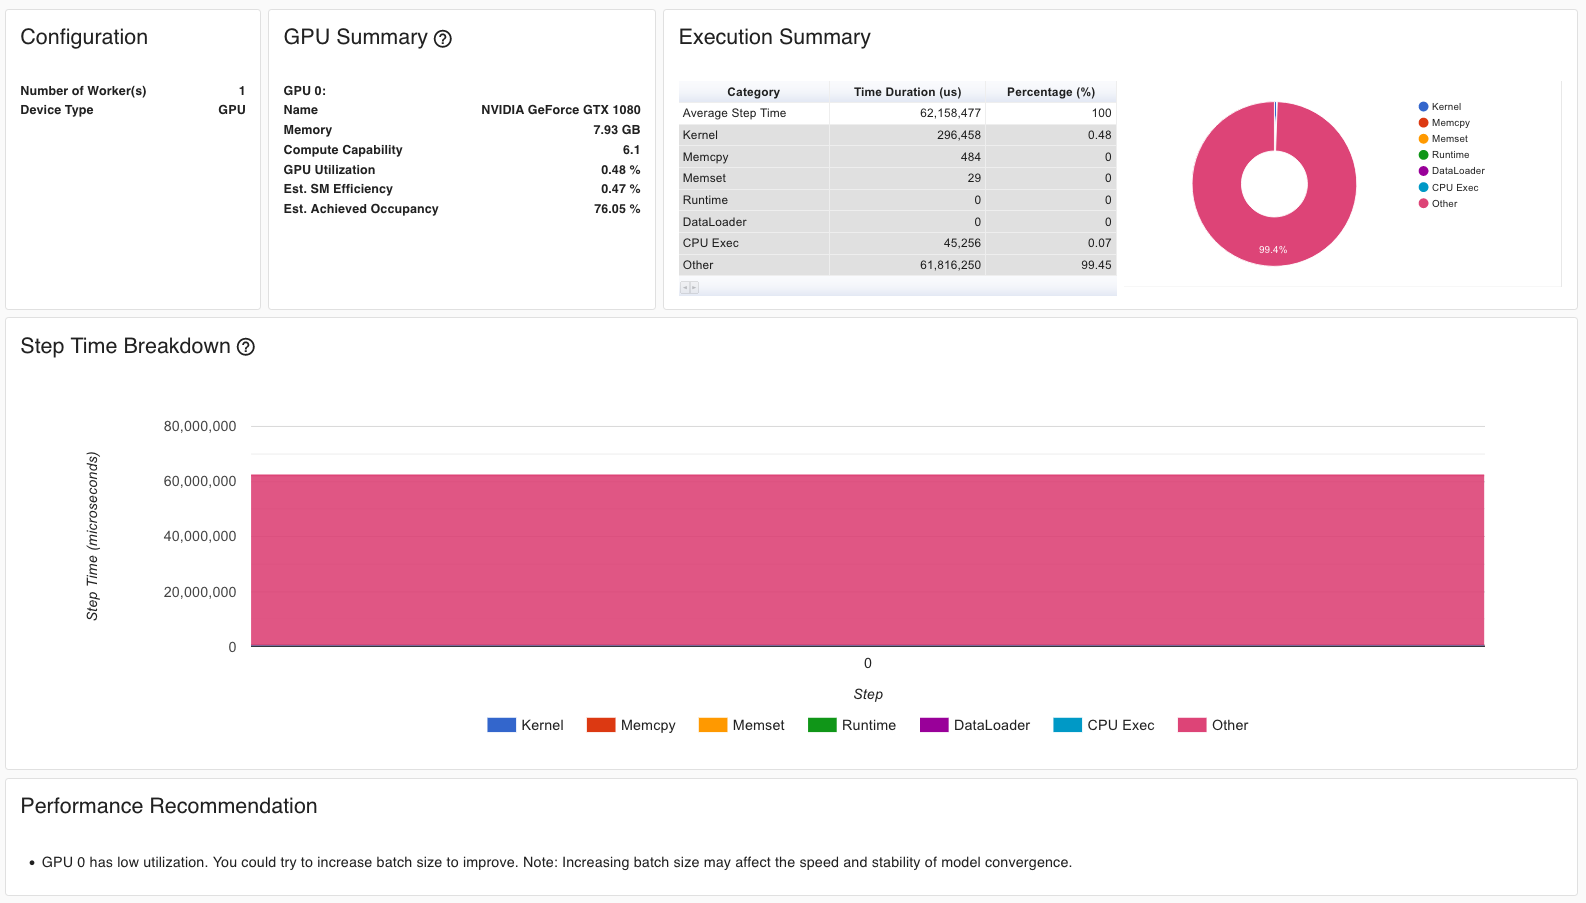
\includegraphics[width=1\textwidth]{../../data/scap_gtx1080_profiler-torch_sample-points_14628864}
    \end{figure}
    \end{center}
\end{frame}

\begin{frame}{Trying to use the PyTorch Profiler to find the reason}
    \begin{center}
    \begin{figure}
        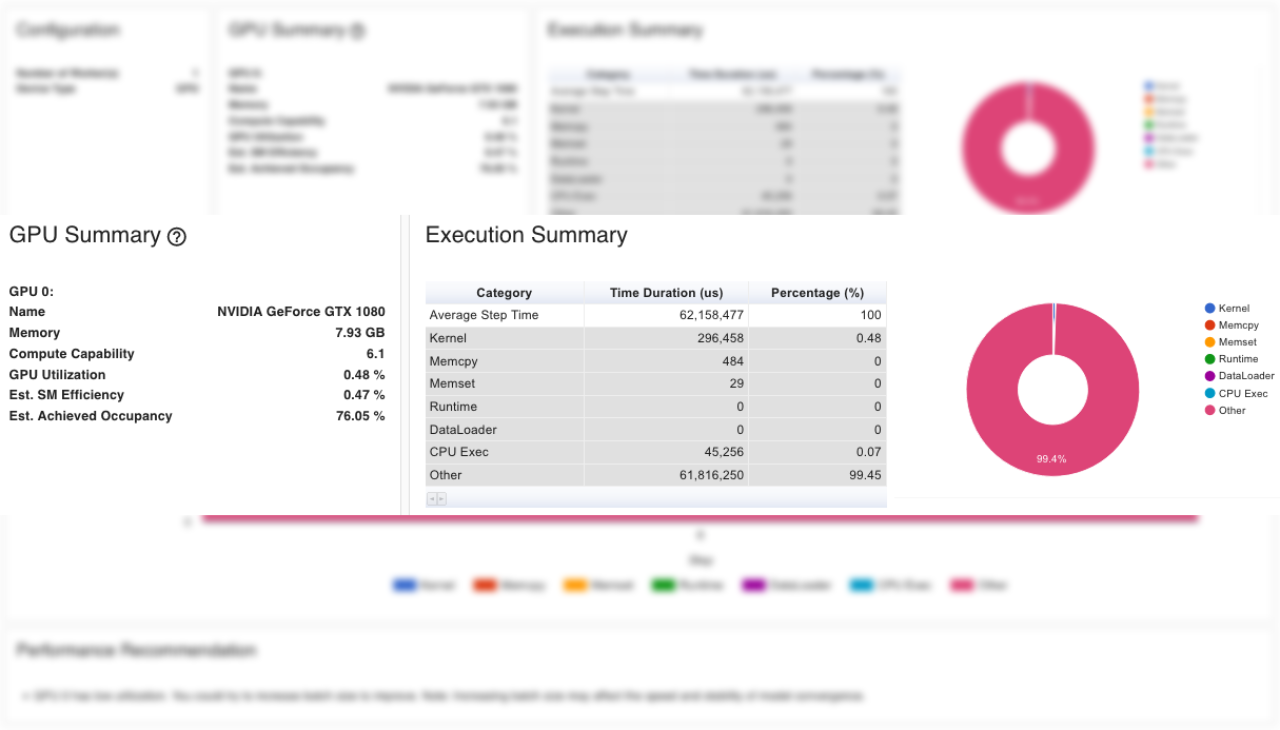
\includegraphics[width=1\textwidth]{../../data/scap_gtx1080_profiler-torch_sample-points_14628864_zoom}
    \end{figure}
    \end{center}
\end{frame}

\begin{frame}{Without help of profiler: identified data loader as bottleneck}
    
\end{frame}

\begin{frame}{Effect of sample points}
    \vspace{-1em}
    \begin{center}
    \begin{figure}
        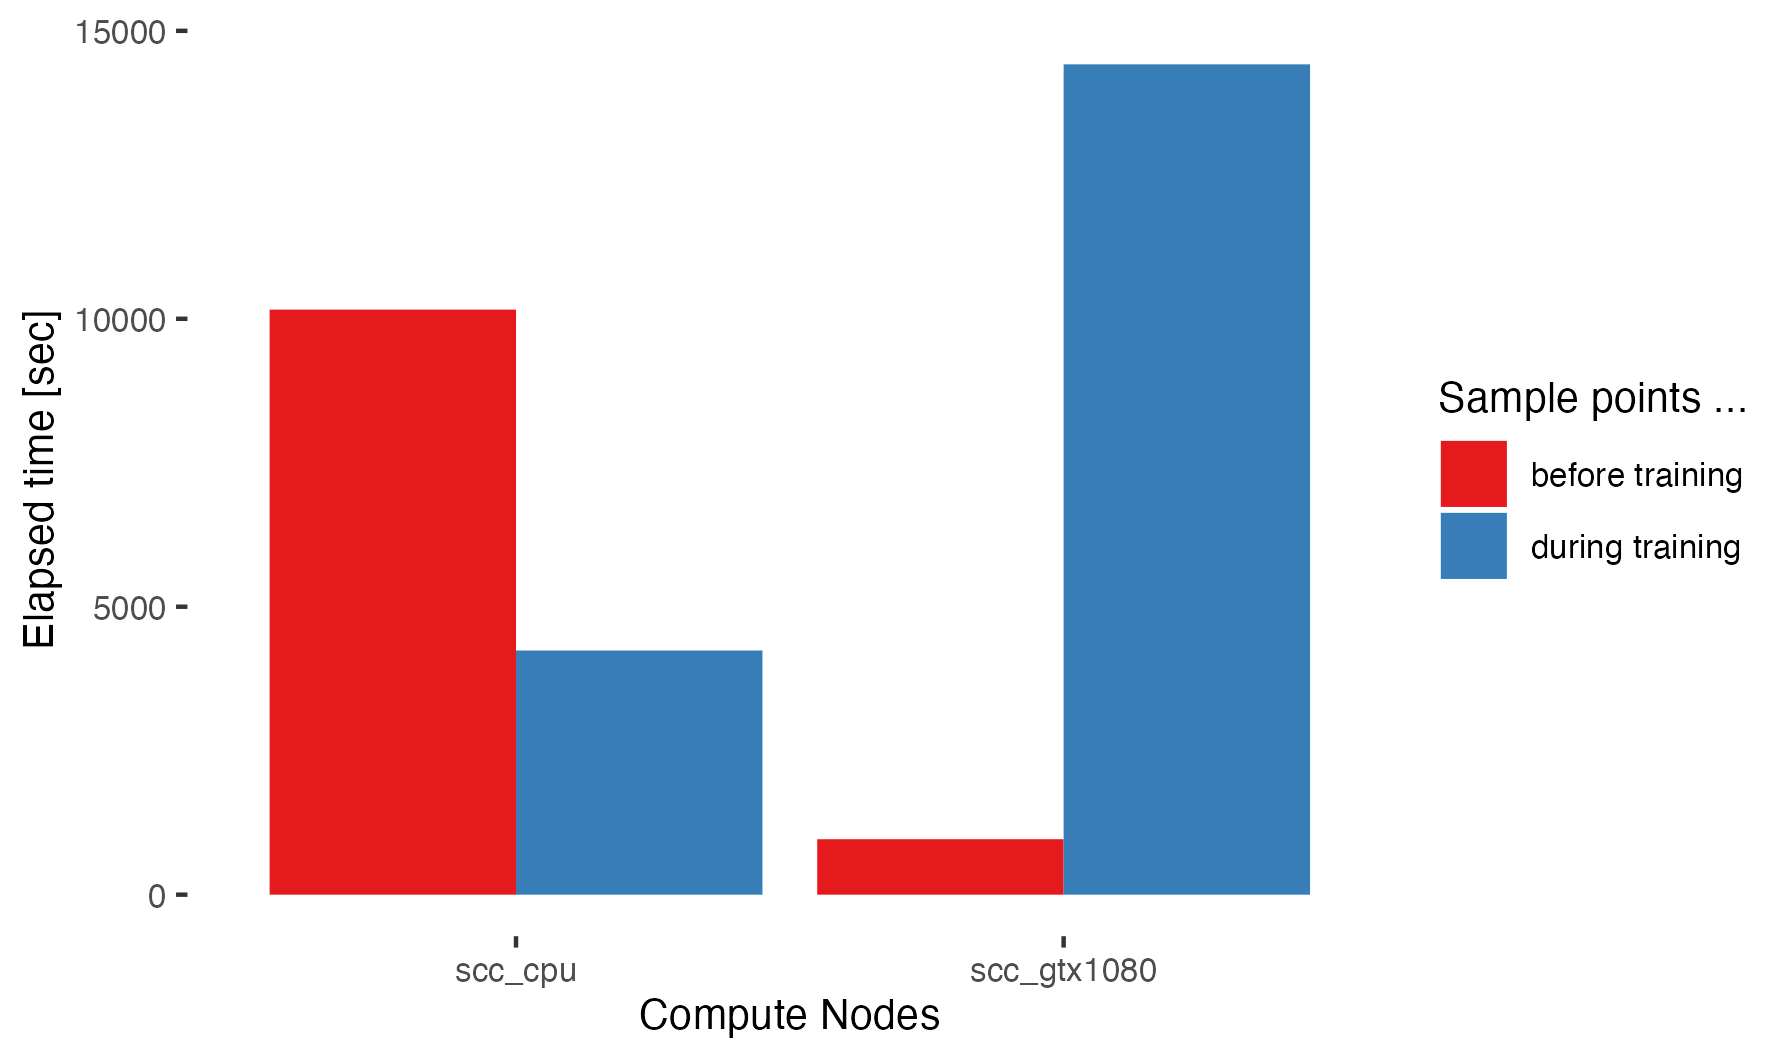
\includegraphics[width=0.85\textwidth]{../../data/sacct_barplot_by_nodes_sample-points-effect}
    \end{figure}
    \end{center}
\end{frame}


\begin{frame}{Test runs}
\label{pg:lastpage} % Label on last frame to get the page number for footer

\begin{columns}
        \begin{column}{0.5\textwidth}
            \centering
            \vspace{-1em}
            \begin{figure}
            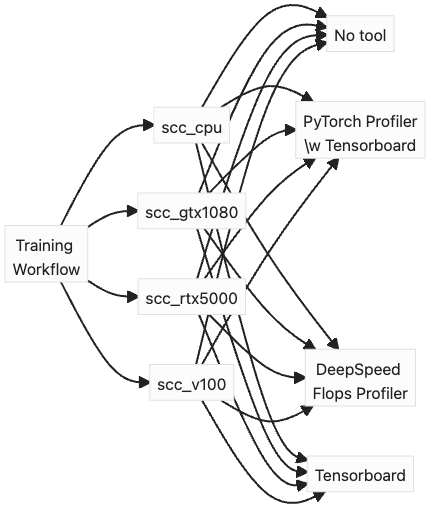
\includegraphics[width=0.85\textwidth]{../../data/runs.png}
            \caption*{abc}
            \end{figure}
        \end{column}
        \begin{column}{0.5\textwidth}
            \begin{itemize}
                \item "Stable Diffusion v1 version of the model requires 150,000 A100 GPU Hours for a single training session"\footnote{\tiny{\url{https://syncedreview.com/2022/11/09/almost-7x-cheaper-colossal-ais-open-source-solution-accelerates-aigc-at-a-low-cost-diffusion-pretraining-and-hardware-fine-tuning-can-be/}}, accessed on: 10.11.2022}
                \vspace{1em}
                \item[$\Rightarrow$] Optimization of deep learning workflows is of growing importance for energy efficiency.
            \end{itemize}
        \end{column}
    \end{columns}

\end{frame}

\begin{frame}{Test runs - table}
% Please add the following required packages to your document preamble:
% \usepackage{booktabs}
\begin{table}[]
\resizebox{1.2\textheight}{!}{
\begin{tabular}{@{}llllll@{}}
\toprule
run & node         & tool           & job\_id  & is\_valid & experiment    \\ \midrule
1   & scc\_cpu     & no-tool        &          & TRUE      &               \\
2   & scc\_cpu     & tensorboard    &          & TRUE      &               \\
3   & scc\_cpu     & profiler-torch & 14629425 & TRUE      &               \\
4   & scc\_cpu     & deepspeed      & 14617521 & FALSE     &               \\
5   & scc\_gtx1080 & no-tool        & 14619617 & TRUE      &               \\
6   & scc\_gtx1080 & tensorboard    & 14615343 & TRUE      &               \\
7   & scc\_gtx1080 & profiler-torch & 14615562 & TRUE      &               \\
8   & scc\_gtx1080 & deepspeed      & 14615344 & TRUE      &               \\
9   & scc\_rtx5000 & no-tool        & 14619618 & TRUE      &               \\
10  & scc\_rtx5000 & tensorboard    & 14617172 & TRUE      &               \\
11  & scc\_rtx5000 & profiler-torch & 14617173 & TRUE      &               \\
12  & scc\_rtx5000 & deepspeed      & 14617171 & TRUE      &               \\
13  & scc\_v100    & no-tool        & 14619619 & TRUE      &               \\
14  & scc\_v100    & tensorboard    & 14617203 & TRUE      &               \\
15  & scc\_v100    & profiler-torch & 14617204 & TRUE      &               \\
16  & scc\_v100    & deepspeed      & 14617202 & TRUE      &               \\
17  & scc\_gtx1080 & profiler-torch & 14629008 & TRUE      & batch-size-64 \\
18  & scc\_gtx1080 & profiler-torch & 14628864 & TRUE      & sample-points \\
19  & scc\_cpu     & profiler-torch & 14629422 & TRUE      & sample-points \\ \bottomrule
\end{tabular}
}
\end{table}
\end{frame}

\begin{frame}{Overview - runtime on HPC}
    \vspace{-1.35em}
    \begin{center}
    \begin{figure}
        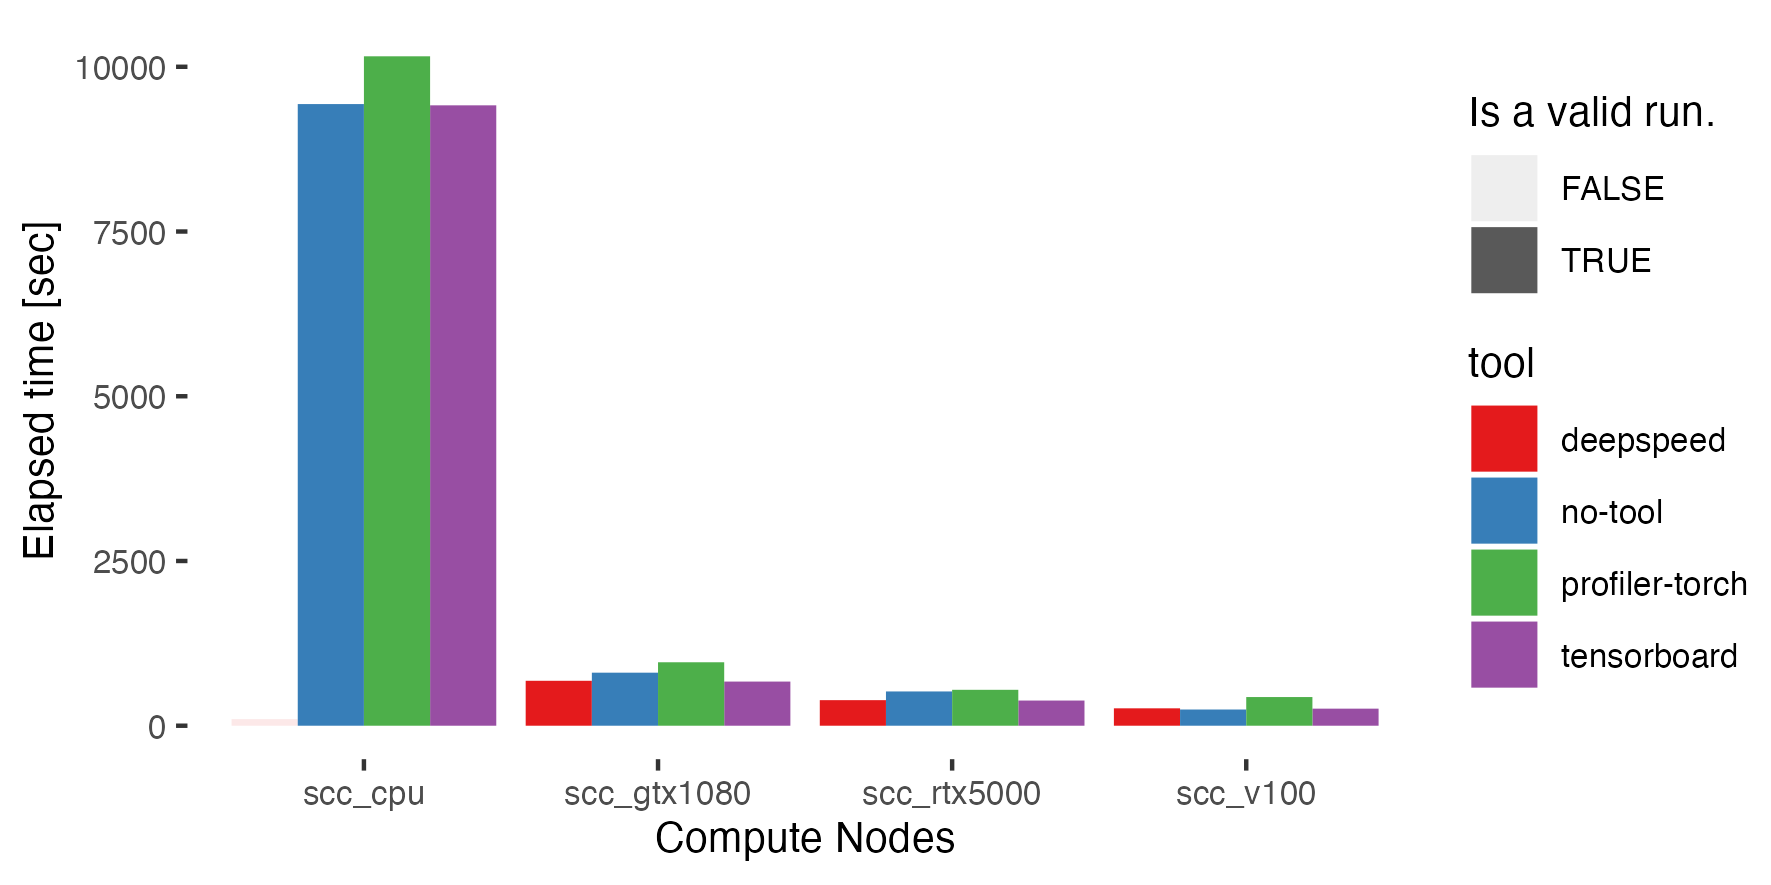
\includegraphics[width=1\textwidth]{../../data/sacct_barplot_by_nodes_no-experiment}
    \end{figure}
    \end{center}
\end{frame}

\begin{frame}{Overview - runtime on HPC - GPU-only}
    \vspace{-1.35em}
    \begin{center}
    \begin{figure}
        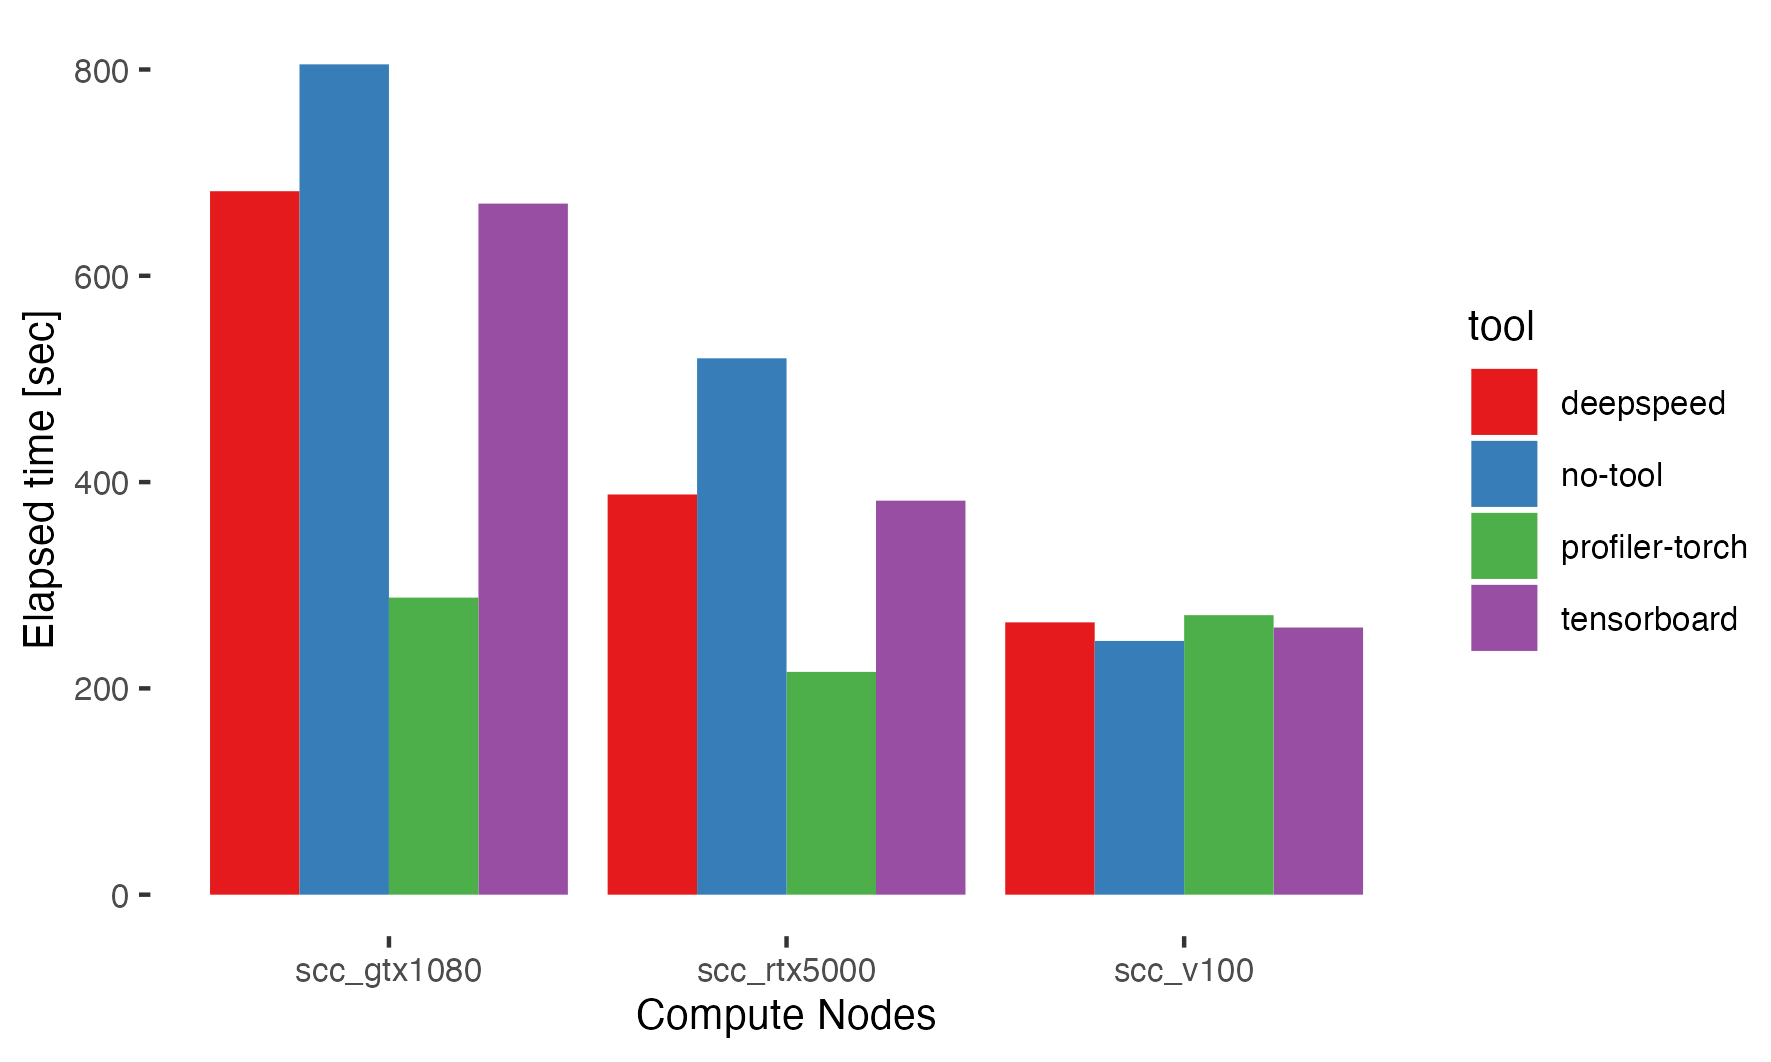
\includegraphics[width=0.9\textwidth]{../../data/sacct_barplot_by_nodes_no-experiment_gpu}
    \end{figure}
    \end{center}
\end{frame}

\begin{frame}{Until now everything was achieved with sacct}

    \begin{listings}
sacct --format=jobid,elapsed -P -j 14629422,14617521,14615343,14615562,14615344,14617172,14617173,\
14617171,14618941,14617203,14619619,14617204,14619618,14619617,\
14617202,14628864,14629008,14629421,14629426,14629425 -X


    JobID|Elapsed
14615343|00:11:10
14615344|00:11:22
14615562|00:04:48
14617171|00:06:28
14617172|00:06:22
14617173|00:03:36
14617202|00:04:24
14617203|00:04:19
14617204|00:04:31
14617521|00:01:40
14618941|00:20:02
14619617|00:13:25
14619618|00:08:40
14619619|00:04:06
14628864|01:07:19
14629008|00:06:45
14629421|02:37:14
14629422|01:10:40
14629425|00:13:55
14629426|02:36:55
\end{listings}

\end{frame}


\begin{frame}{lets look at the pytorch profiler hint section}

\begin{center}
    \begin{figure}
        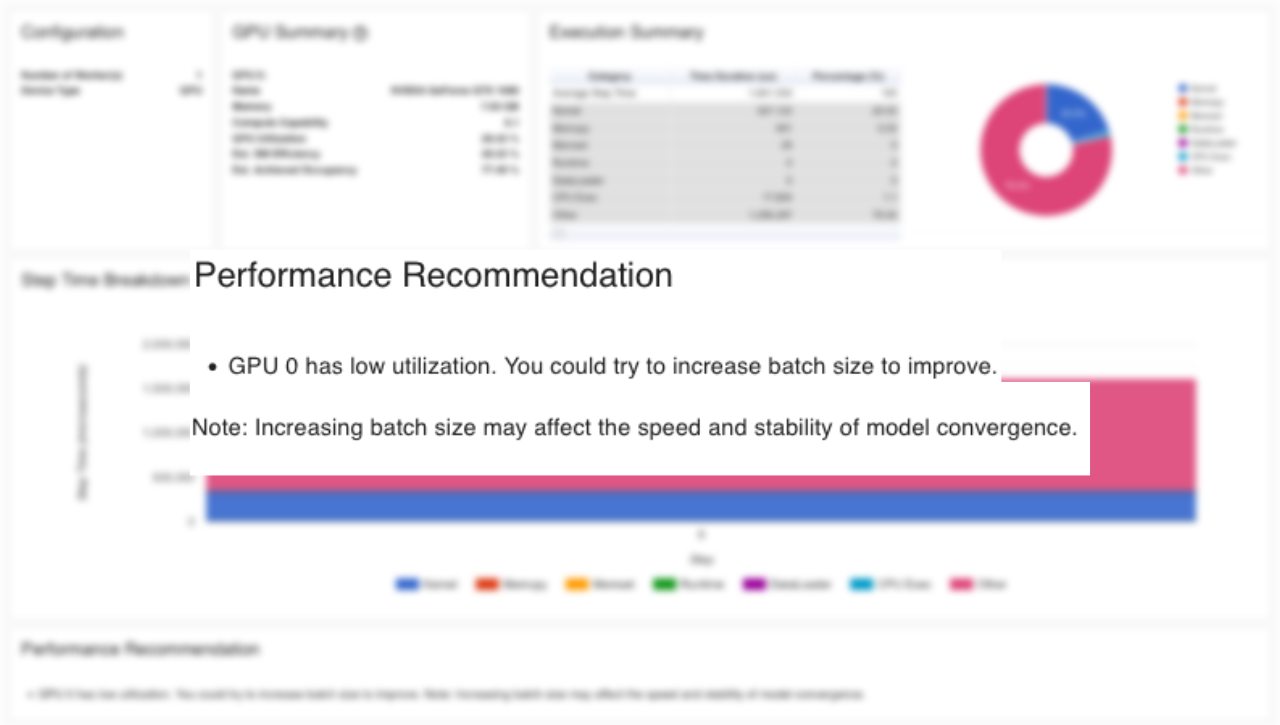
\includegraphics[width=1\textwidth]{../../data/scap_gtx1080_profiler-torch_14615562}
    \end{figure}
\end{center}

\end{frame}

\begin{frame}{lets look at the pytorch profiler hint section}

\begin{center}
    \begin{figure}
        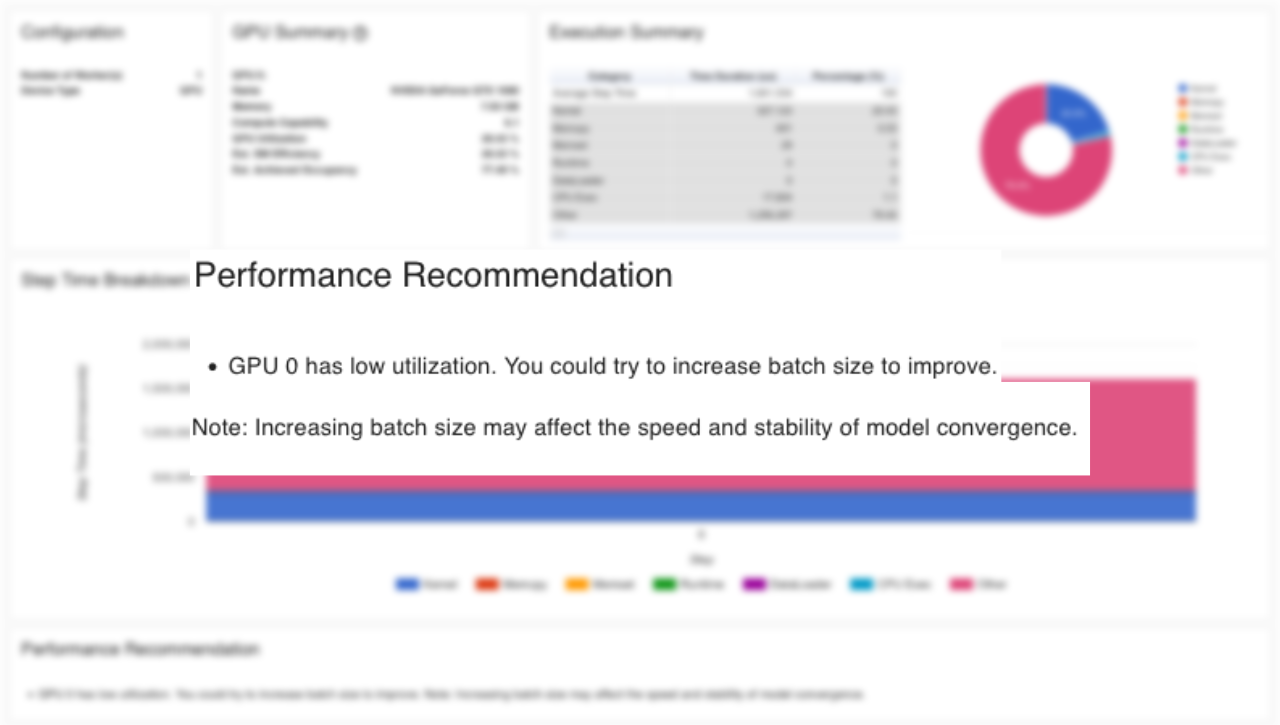
\includegraphics[width=1\textwidth]{../../data/scap_gtx1080_profiler-torch_14615562_zoom}
    \end{figure}
\end{center}

\end{frame}

\begin{frame}{result of increasing batch size - 64}

\begin{center}
    \begin{figure}
        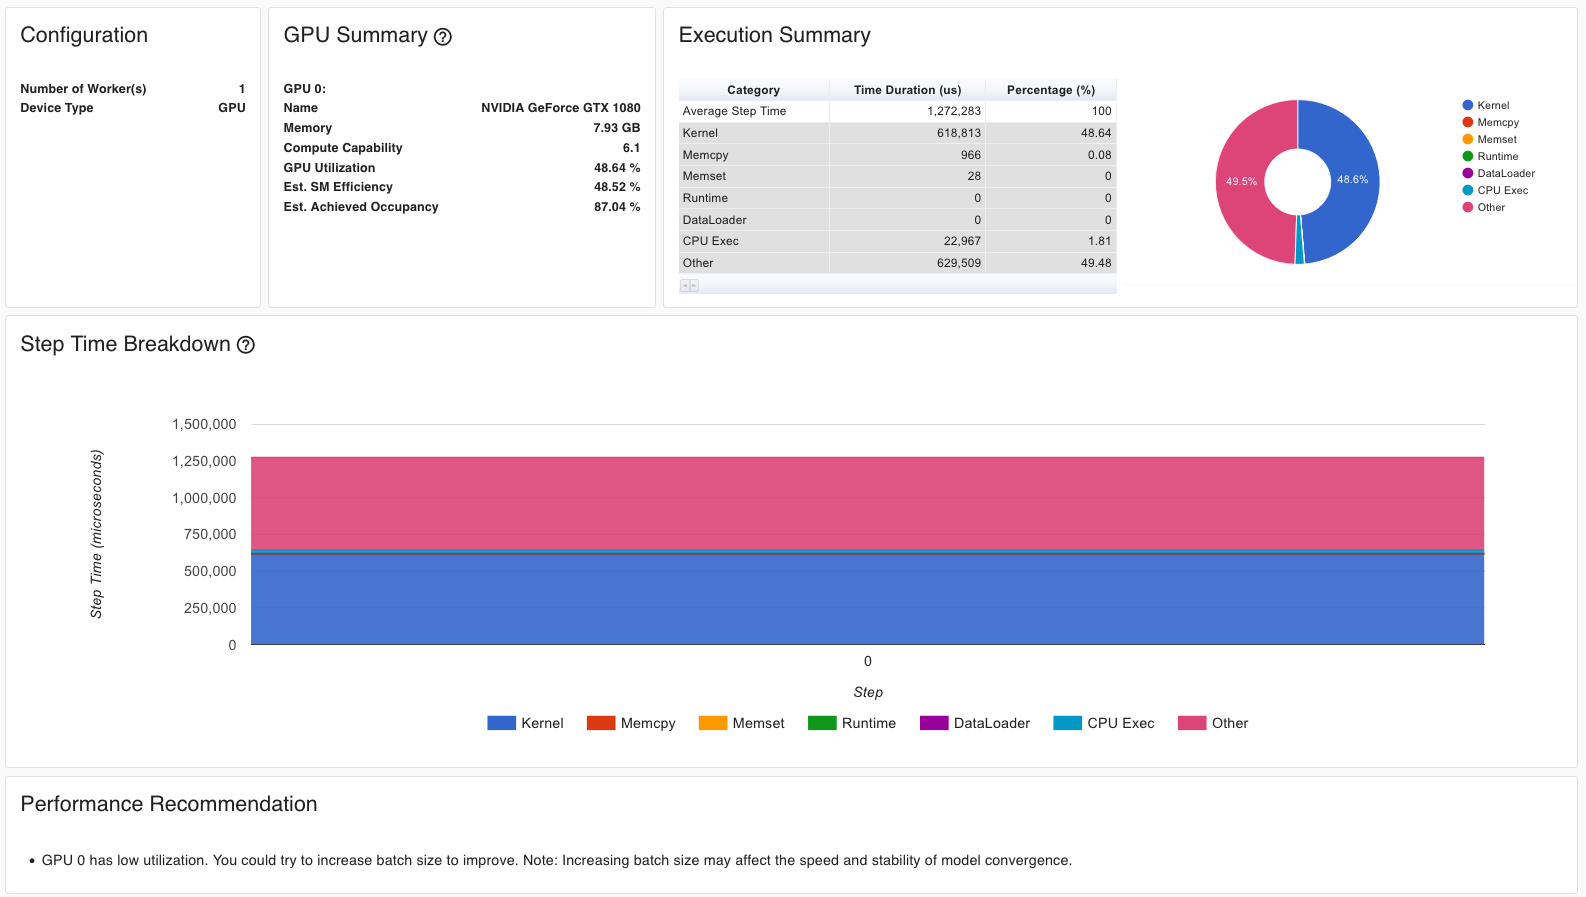
\includegraphics[width=1\textwidth]{../../data/scap_gtx1080_profiler-torch_batch-size-64_14629008}
    \end{figure}
    \end{center}

\end{frame}

\begin{frame}{result of increasing batch size - 64}

\begin{center}
    \begin{figure}
        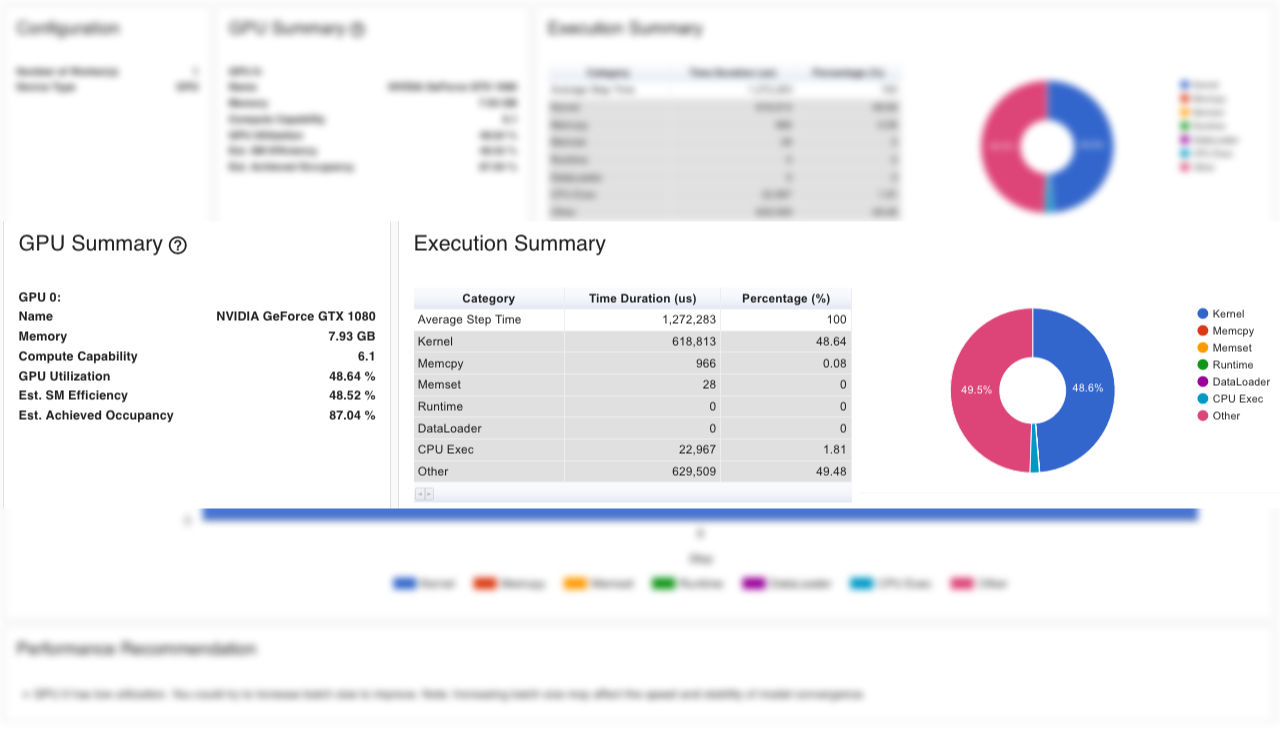
\includegraphics[width=1\textwidth]{../../data/scap_gtx1080_profiler-torch_batch-size-64_14629008_zoom}
    \end{figure}
    \end{center}

\end{frame}


\begin{frame}{result of increasing batch size - 128}

\begin{center}
    \begin{figure}
        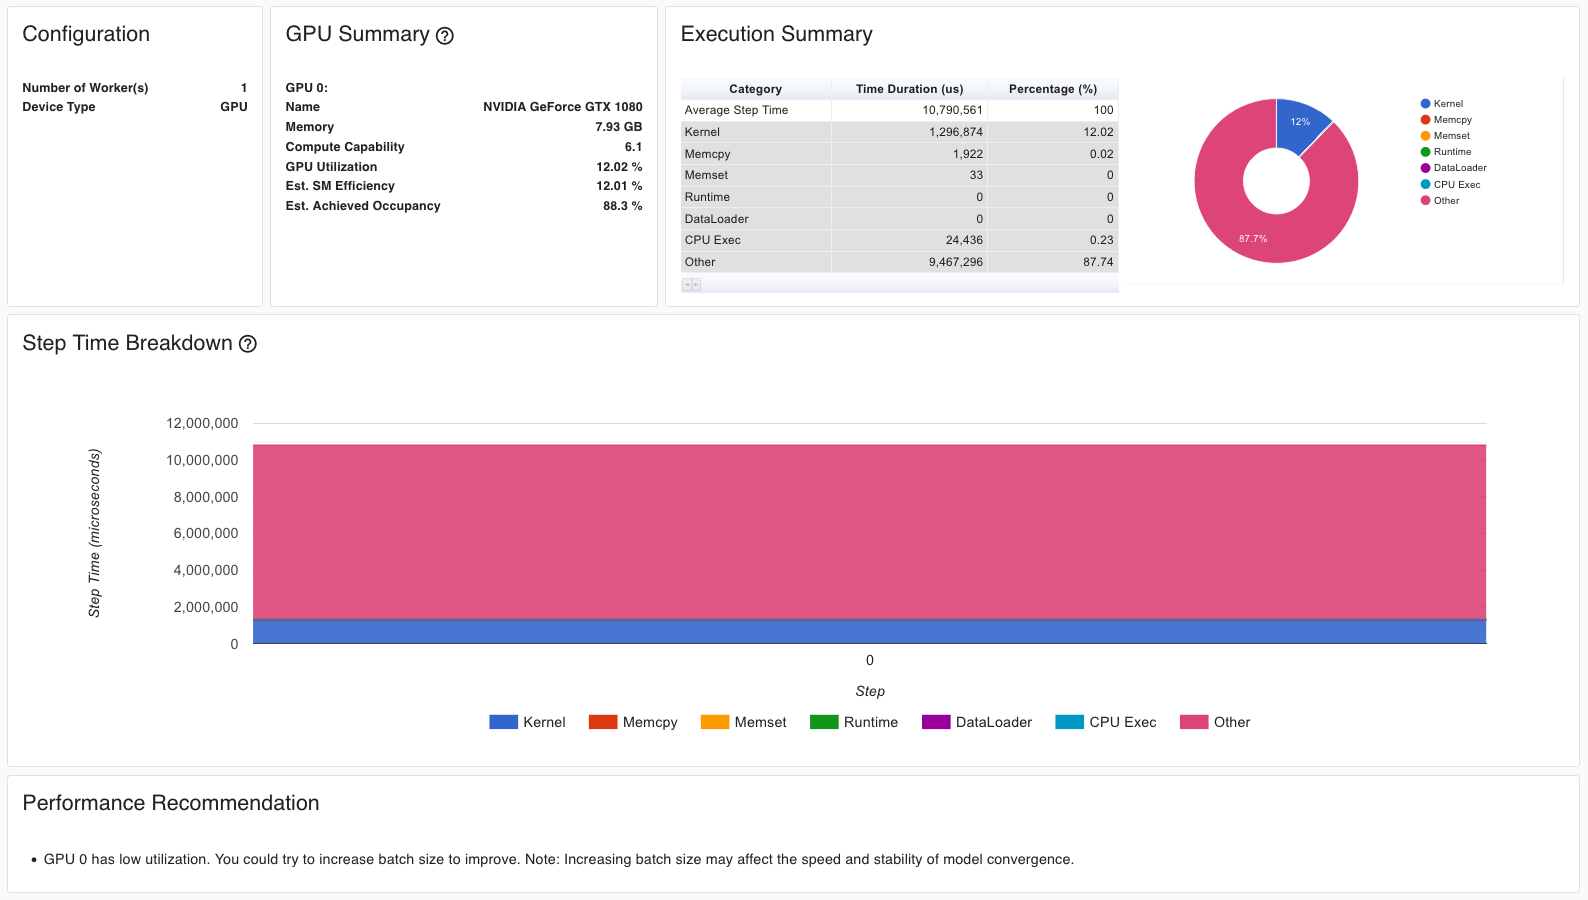
\includegraphics[width=1\textwidth]{../../data/scap_gtx1080_profiler-torch_batch-size-128_14633534}
    \end{figure}
    \end{center}

\end{frame}

\begin{frame}{result of increasing batch size - 128}

\begin{center}
    \begin{figure}
        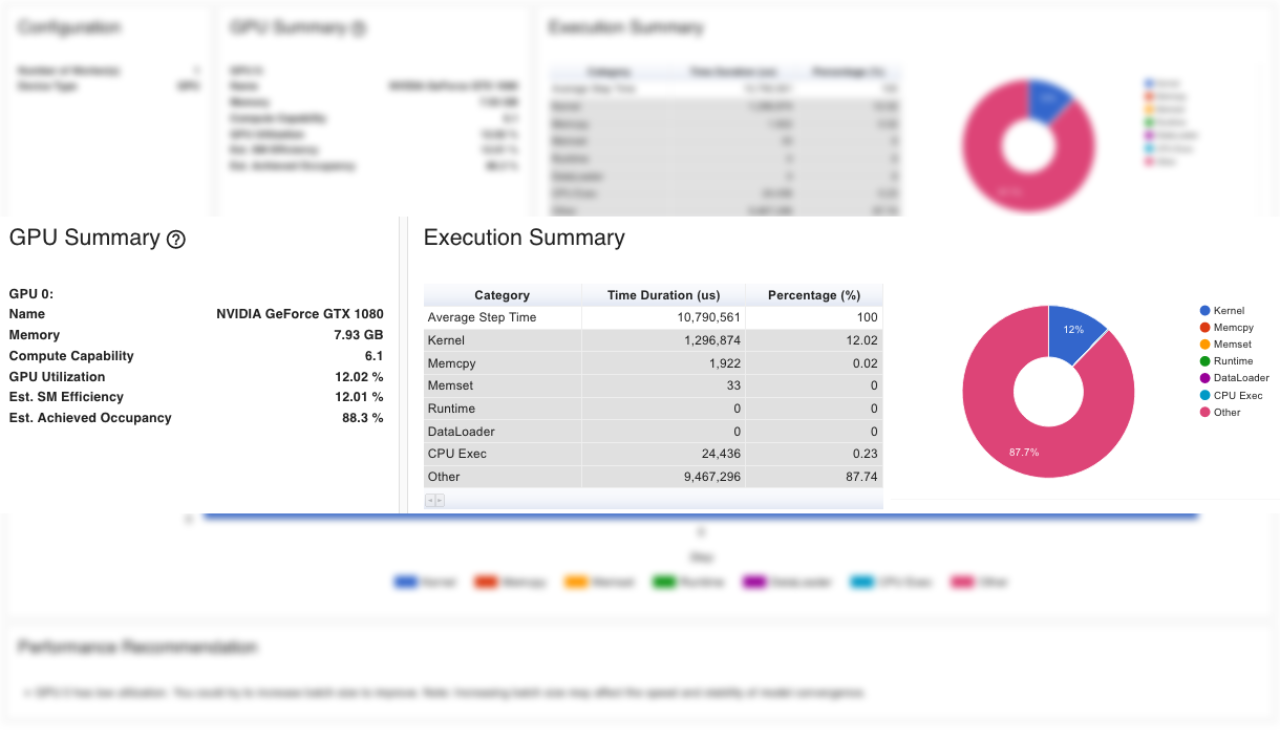
\includegraphics[width=1\textwidth]{../../data/scap_gtx1080_profiler-torch_batch-size-128_14633534_zoom}
    \end{figure}
    \end{center}

\end{frame}

\begin{frame}{result of increasing batch size}
    \vspace{-1em}
    \begin{center}
        \begin{figure}
            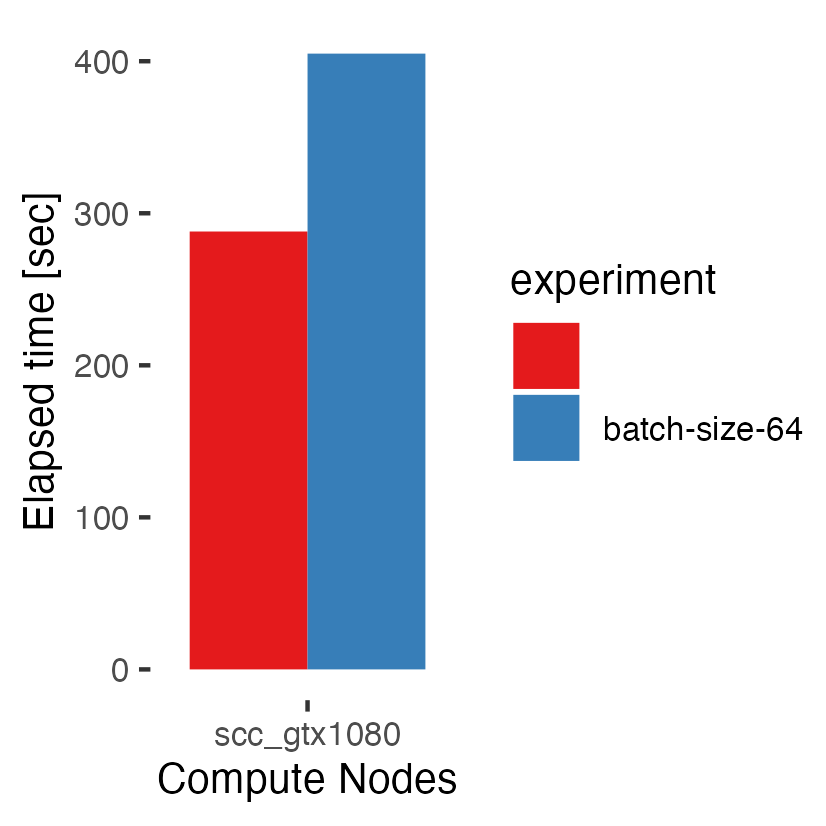
\includegraphics[width=0.85\textwidth]{../../data/sacct_barplot_by_nodes_batch-size-effect}

        \end{figure}
    \end{center}
\end{frame}

%%%%%%%%%%%%%%%%

\begin{frame}{Benchmarking is the first step of optimizing}
\label{pg:lastpage} % Label on last frame to get the page number for footer

\begin{columns}
        \begin{column}{0.5\textwidth}
            \centering
            \vspace{-1em}
            \begin{figure}
            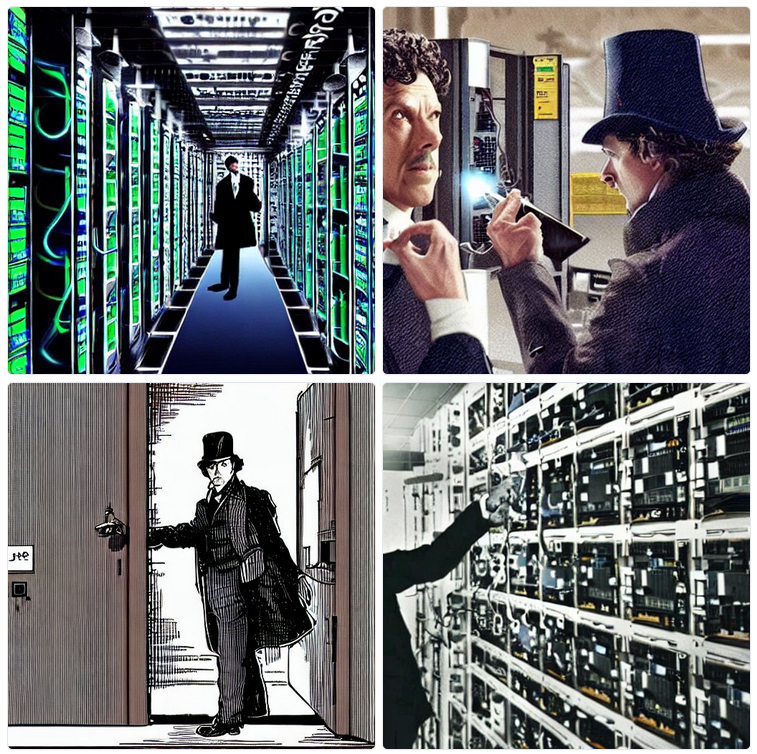
\includegraphics[width=0.85\textwidth]{assets/Sherlock-Holmes-locates-the-best-graphical-processing-unit-inside-the-data-center-for-his-deep-learning-workflow}
            \caption*{Image generated with stable diffusion: \\
            \tiny{"Sherlock Holmes locates the best graphical processing unit inside the data center for his deep learning workflow"}}
            \end{figure}
        \end{column}
        \begin{column}{0.5\textwidth}
            \begin{itemize}
                \item "Stable Diffusion v1 version of the model requires 150,000 A100 GPU Hours for a single training session"\footnote{\tiny{\url{https://syncedreview.com/2022/11/09/almost-7x-cheaper-colossal-ais-open-source-solution-accelerates-aigc-at-a-low-cost-diffusion-pretraining-and-hardware-fine-tuning-can-be/}}, accessed on: 10.11.2022}
                \vspace{1em}
                \item[$\Rightarrow$] Optimization of deep learning workflows is of growing importance for energy efficiency.
            \end{itemize}
        \end{column}
    \end{columns}

\end{frame}

\begin{frame}{References}
    % References slide in appendix
    \renewcommand*{\bibfont}{\normalfont\scriptsize}
    \printbibliography[heading=none]
\end{frame}

\end{document}
